\documentclass[11pt]{report}

\usepackage[a4paper,margin=1in]{geometry}
\usepackage[utf8]{inputenc}
\usepackage[T1]{fontenc}
\usepackage[strings]{underscore}
\usepackage{graphicx}
\usepackage{booktabs}
\usepackage{longtable}
\usepackage{array}
\usepackage{caption}
\usepackage{listings}
\usepackage{xcolor}
\usepackage{hyperref}
\usepackage{amsmath}
\usepackage{enumitem}
\usepackage{tabularx}
\usepackage{fancyhdr}
\usepackage{float}

\graphicspath{{results/figures/}}
\hypersetup{colorlinks=true, linkcolor=blue, citecolor=blue, urlcolor=blue}

\lstdefinestyle{pystyle}{
  language=Python,
  basicstyle=\ttfamily\footnotesize,
  keywordstyle=\color{blue},
  commentstyle=\color{gray},
  stringstyle=\color{teal},
  numbers=left,
  numberstyle=\tiny\color{gray},
  breaklines=true,
  breakatwhitespace=false,
  frame=single,
  showstringspaces=false,
  tabsize=4,
  columns=flexible,
}
\lstset{style=pystyle}

\pagestyle{fancy}
\fancyhf{}
\fancyhead[L]{DEAP Comparative Analysis --- Project Report}
\fancyhead[R]{\thepage}

\title{DEAP EEG Emotion Recognition: A Comparative Analysis of\\
Classical and Deep Learning Pipelines\\
\large Project Report --- Methodology, Code Walkthrough, Literature\\
Attribution, and Findings}
\author{Koustav Das}
\date{\today}

\begin{document}

\maketitle
\tableofcontents
\listoffigures
\listoftables

\chapter{Introduction and Objectives}

\section{Purpose of this report}
This document is a complete technical record of the work carried out in the
\texttt{D:\textbackslash EEG} project: a head-to-head comparison of two
feature/modeling paradigms for binary emotion classification on the DEAP
dataset, followed by an extended, eighteen-section investigation into why
subject-independent performance on this dataset is weak, and a final
cross-corpus validation against SEED-IV. It is written so that it can be
expanded into a formal report or thesis chapter: every notebook section,
every standalone Python script, every literature source consulted, and every
open/unresolved item is documented here with enough detail to reconstruct the
reasoning behind each design decision.

\section{Objectives}
\begin{enumerate}
  \item Build two parallel, directly-comparable pipelines for classifying
        DEAP's four emotion dimensions (valence, arousal, dominance, liking)
        from EEG: a classical-ML pipeline on hand-crafted Differential
        Entropy (DE) band-power features (\textbf{Track A}), and a
        deep-learning pipeline on raw, baseline-normalized EEG windows
        (\textbf{Track B}).
  \item Evaluate both under a genuinely \textbf{subject-independent}
        protocol (\texttt{GroupKFold} / \texttt{GroupShuffleSplit}, grouped
        by subject) rather than the leakier, ungrouped splits common in the
        published literature.
  \item If subject-independent performance turns out to be weak, exhaustively
        test plausible causes: feature richness, hyperparameter tuning, CV
        rigor, data quantity (window overlap), label definition, per-subject
        calibration, feature/distribution alignment, adversarial
        subject-invariance, self-supervised pretraining, an AUC-targeted
        loss, test-time adaptation, and diagnostic interpretability (SHAP).
  \item Validate whether the resulting near-chance ceiling is a property of
        DEAP specifically, or of subject-independent EEG emotion decoding in
        general, via genuine cross-corpus transfer to a second dataset
        (SEED-IV).
  \item Ground every claim in a literature review of 32 papers assembled in
        \texttt{D:\textbackslash EEG\textbackslash papers\_EEG\textbackslash},
        and report honestly wherever an intervention did \emph{not} help.
\end{enumerate}

\section{How this report is organised}
Chapter~\ref{ch:dataset} describes the DEAP dataset and the two evaluation
datasets involved (DEAP itself and SEED-IV). Chapter~\ref{ch:repo} maps the
repository layout. Chapter~\ref{ch:notebook} is the core of the report: a
section-by-section walkthrough of every cell in
\texttt{DEAP\_Comparative\_Analysis.ipynb}, explaining what each code block
does and why. Chapter~\ref{ch:scripts} documents every standalone
\texttt{scripts/*.py} file. Chapter~\ref{ch:literature} is the literature
review and paper-attribution table. Chapter~\ref{ch:results} consolidates the
numeric results. Chapters~\ref{ch:done}--\ref{ch:challenges} cover what was
accomplished, what was left undone, what could have been done differently,
and the concrete challenges encountered. Chapter~\ref{ch:conclusion}
concludes.

\chapter{Dataset and Problem Setup}
\label{ch:dataset}

\section{DEAP}
The DEAP dataset (\texttt{data\_preprocessed\_python}) contains 32 subjects
$\times$ 40 trials $\times$ 32 EEG channels sampled at 128\,Hz. Each subject
file \texttt{sXX.dat} is a pickled dictionary with:
\begin{itemize}
  \item \texttt{data}: shape $(40, 40, 8064)$ --- 40 trials, the first 32 of
        40 channels are EEG (the remaining 8 are peripheral physiological
        signals, dropped throughout this project). 8064 samples = 3\,s
        pre-trial baseline (384 samples) + 60\,s of stimulus (7680 samples).
  \item \texttt{labels}: shape $(40, 4)$ --- continuous 1--9 self-assessment
        ratings for valence, arousal, dominance, and liking.
\end{itemize}
Labels are binarised at the DEAP-standard threshold of 5.0 (rating $>5 \Rightarrow$
class 1). Section~\ref{sec:s4} shows this binarisation is \textbf{not}
balanced: valence is 21.0\%/79.0\%, arousal 23.3\%/76.7\%, dominance
60.9\%/39.1\%, and liking 66.5\%/33.5\% high/low -- a fact that turns out to
explain a large share of this project's most important methodological
finding (Section~\ref{sec:s8}).

\section{SEED-IV}
SEED-IV (Zheng, Liu, Cheng \& Lu, 2018, ``EmotionMeter'') is used as the
cross-corpus validation target in Section~\ref{sec:s12}. It shares SEED's
62-channel montage and 15 subjects, but differs from the original 3-class
SEED dataset in several respects that required a dedicated adapter
(Section~\ref{sec:seed-iv-adapter}): 4 emotion classes (0 = neutral,
1 = sad, 2 = fear, 3 = happy) instead of 3; 24 film-clip trials per session
instead of 15; 3 sessions per subject, each with its \emph{own} trial-label
order (unlike original SEED's single shared label file); and raw trials of
variable duration (tens of thousands of samples at 200\,Hz) rather than
DEAP's fixed 60\,s. SEED-IV was chosen over original SEED specifically
because it is mirrored on Kaggle
(\url{https://www.kaggle.com/datasets/phhasian0710/seed-iv}) without a
signed data-use agreement, whereas original SEED, DREAMER, and AMIGOS all
remain gated behind such agreements (see Chapter~\ref{ch:not-done}).

\chapter{Repository Structure}
\label{ch:repo}

\begin{verbatim}
D:\EEG
|-- DEAP_Comparative_Analysis.ipynb   (the main notebook; 88 cells, 18+ sections)
|-- deap-dataset\data_preprocessed_python\   (raw DEAP .dat files, 32 subjects)
|-- seed-dataset\                     (SEED-IV download: eeg_raw_data/{1,2,3}/, etc.)
|-- processed_cache\                  (cached .npz feature/window builds)
|-- results\
|   |-- tables\   (21 CSV result tables)
|   \-- figures\  (23+ PNG figures)
|-- papers_EEG\   (32 literature-review PDFs, renamed to descriptive titles)
\-- scripts\
    |-- dl_models.py, rich_features.py
    |-- build_extended_features.py, build_overlap_windows.py, build_raw_ratings.py
    |-- track_a_*.py   (9 classical-ML companion experiments)
    |-- track_b_*.py   (5 deep-learning companion experiments)
    |-- update_notebook*.py  (historical notebook-authoring/generation scripts)
    \-- cross_corpus\
        |-- base.py, seed_adapter.py, run_cross_corpus.py, README.md
\end{verbatim}

The notebook is the primary deliverable; the \texttt{scripts/} directory holds
every experiment that was too expensive to run inline (most of Sections
9--18), each of which writes its results to a CSV in
\texttt{results/tables/}, which the notebook then reads and plots. This
split is deliberate and is discussed further in Chapter~\ref{ch:challenges}.

\chapter{Notebook Walkthrough}
\label{ch:notebook}

This chapter explains every section and code cell of
\texttt{DEAP\_Comparative\_Analysis.ipynb} in the order they appear. The
notebook was executed end-to-end in a real Jupyter kernel (37 code cells,
sequential execution counts 1--37, zero errors, 15.6 minutes total wall
time), so every number quoted below is a genuine, reproducible output
(\texttt{SEED = 42} fixes all randomness in scikit-learn/XGBoost/PyTorch/NumPy).

\section{Section 1 -- Configuration \& Environment}
\textbf{Cell (imports)}: imports the full stack --- \texttt{numpy},
\texttt{pandas}, \texttt{matplotlib}/\texttt{seaborn} (theme:
\texttt{whitegrid}, DPI 110), \texttt{scipy.signal} (Butterworth filtering),
\texttt{sklearn} (models, \texttt{GroupKFold}/\texttt{GroupShuffleSplit},
metrics), \texttt{xgboost}, and \texttt{torch}. Sets \texttt{SEED = 42} and
seeds \texttt{random}, \texttt{numpy}, and \texttt{torch} (CPU and CUDA).
Detects and prints the GPU (\texttt{NVIDIA GeForce RTX 3070 Ti}, CUDA
available). Defines a fixed, colour-blind-safe categorical palette
(\texttt{PALETTE}) mapping each of the 10 models (6 classical + 4 deep) to
one consistent colour, reused in every plot in the notebook.

\textbf{Cell (config)}: defines \texttt{QUICK\_RUN} (smoke-test switch, unused
in the final run --- all 32 subjects were used), \texttt{DATA\_DIR},
\texttt{CACHE\_DIR}, and \texttt{RESULTS\_DIR} with its two subfolders
\texttt{FIGURES\_DIR}/\texttt{TABLES\_DIR} (auto-created); \texttt{FS = 128},
\texttt{BASELINE\_SEC = 3}, \texttt{TRIAL\_SEC = 60},
\texttt{WINDOW\_SEC = 4} (giving 15 non-overlapping 4\,s windows per 60\,s
trial); the four spectral bands (\texttt{theta 4--8, alpha 8--13, beta
13--30, gamma 30--45\,Hz}); \texttt{LABEL\_THRESHOLD = 5.0}; the full
32-channel DEAP 10-20 montage order (used later for TSception's hemisphere
pairing); and \texttt{N\_EPOCHS = 40}, \texttt{BATCH\_SIZE = 128},
\texttt{PATIENCE = 8} for Track B training.

\section{Section 2 -- Loading \& Preprocessing}
\begin{lstlisting}
def load_subject(subject_id):
    fpath = DATA_DIR / f"s{subject_id:02d}.dat"
    with open(fpath, "rb") as f:
        d = pickle.load(f, encoding="latin1")
    return d["data"], d["labels"]

def baseline_normalize(trial_all_channels):
    eeg = trial_all_channels[:N_EEG_CHANNELS]
    baseline = eeg[:, :BASELINE_SAMPLES]
    signal = eeg[:, BASELINE_SAMPLES:BASELINE_SAMPLES + TRIAL_SAMPLES]
    baseline_mean = baseline.mean(axis=-1, keepdims=True)
    return (signal - baseline_mean).astype(np.float64)
\end{lstlisting}
\texttt{baseline\_normalize} subtracts the per-channel mean of the 3\,s
pre-trial baseline from the 60\,s stimulus signal, removing subject/session
DC offset and slow drift before either feature branch is computed.
\texttt{compute\_de\_features} band-pass filters (4th-order Butterworth,
zero-phase \texttt{sosfiltfilt}) into the four bands, reshapes each band into
15 non-overlapping 512-sample windows, and computes the Differential Entropy
of each (channel, band) pair: $\text{DE} = 0.5 \log(2\pi e \, \sigma^2)$,
i.e.\ the closed-form differential entropy of a Gaussian with the window's
own variance $\sigma^2$ --- 32 channels $\times$ 4 bands = 128 features per
window. \texttt{make\_raw\_windows} instead keeps the raw $(32, 512)$ window
and standardises it per-channel (zero mean, unit variance \emph{within that
window}) for stable CNN input. A sanity-check on subject 1's first trial
confirms the expected shapes: \texttt{(15, 128)} DE features and
\texttt{(15, 32, 512)} raw windows.

\section{Section 3 -- Building the Full Windowed Dataset}
Loops over all 32 subjects $\times$ 40 trials, producing \texttt{X\_de}
$(19200, 128)$, \texttt{X\_raw} $(19200, 32, 512)$, one binary label array per
task in \texttt{y\_by\_task}, and a \texttt{groups} array (subject ID per
window, for \texttt{GroupKFold}). Results are cached to
\texttt{processed\_cache/deap\_windows\_4s\_32subj\_v2.npz}
(schema-versioned so stale caches from before dominance/liking were tracked
are never silently reused) --- on a cache hit this cell completes in well
under a second; on a cache miss it takes several minutes.

\section{Section 4 -- Class Balance}
\label{sec:s4}
Bar chart of high/low counts per task. Real numbers (computed directly from
the cached window array, not estimated): \textbf{valence 21.0\% high},
\textbf{arousal 23.3\% high}, \textbf{dominance 60.9\% high},
\textbf{liking 66.5\% high}. Valence and arousal are markedly imbalanced;
dominance and liking are closer to balanced. This chart is flagged in the
notebook's own introduction as something to check before trusting any raw
accuracy number, and that warning turns out to be load-bearing for the
entire rest of the project.

\begin{figure}[H]
\centering
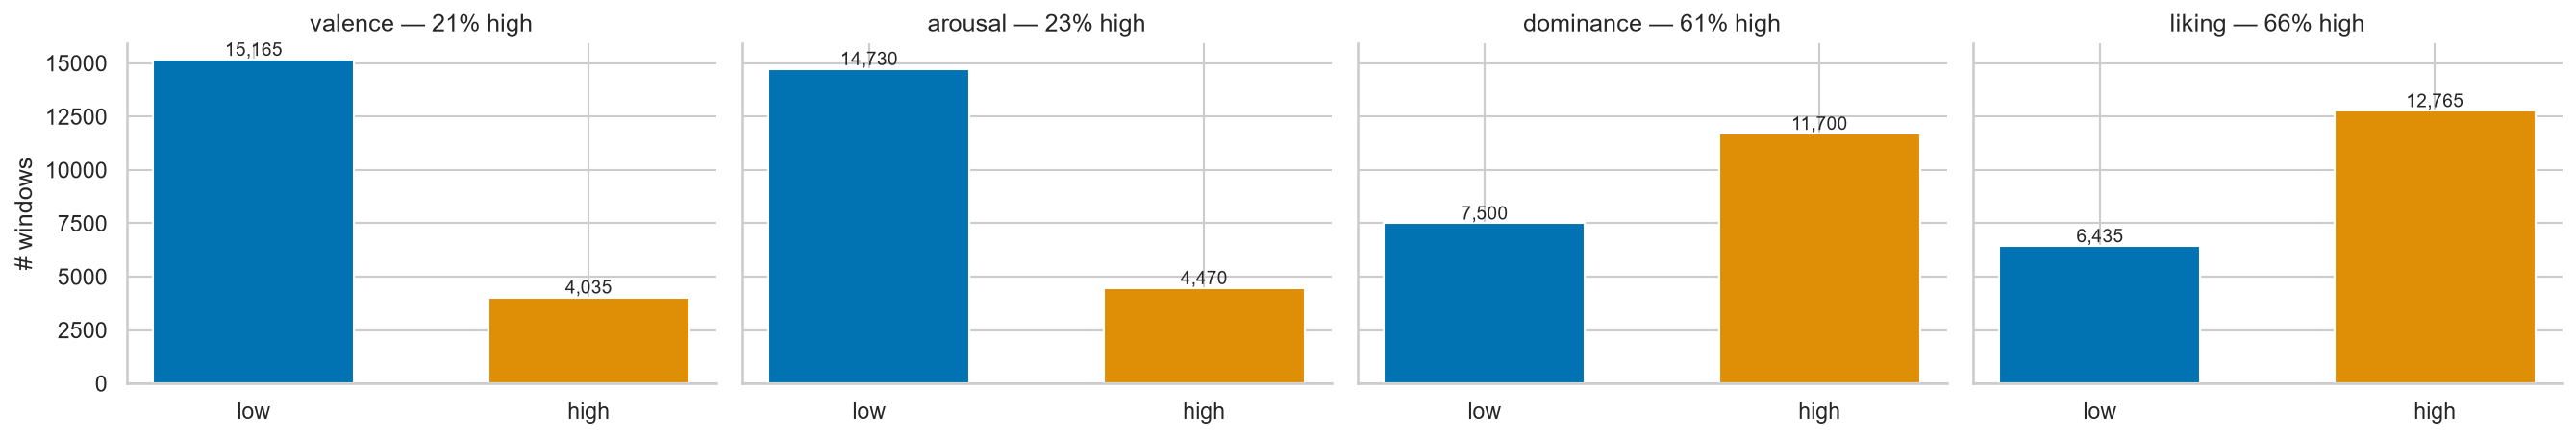
\includegraphics[width=0.8\textwidth]{class_balance.png}
\caption{High/low class balance per task. Valence and arousal are markedly
skewed (21.0\%/79.0\% and 23.3\%/76.7\% high); dominance and liking are
closer to balanced.}
\label{fig:class-balance}
\end{figure}

\section{Section 5 -- Track A: DE Features $\to$ Classical ML}
\label{sec:s5}
Six models (\texttt{LogisticRegression}, \texttt{kNN}, \texttt{RandomForest},
\texttt{SVM-RBF}, \texttt{XGBoost}, \texttt{MLP}), each wrapped in a
\texttt{StandardScaler} pipeline, evaluated with 5-fold \texttt{GroupKFold}
(grouped by subject --- no subject's windows appear in both train and test).
SVM-RBF's training folds are capped at \texttt{SVM\_MAX\_TRAIN\_SAMPLES =
8000} (documented, pragmatic speed trade-off; does not affect the other five
models). Table~\ref{tab:track-a-best} shows the best model per task by
ROC-AUC.

\begin{table}[h]
\centering
\caption{Track A --- best classical model per task (5-fold GroupKFold mean)}
\label{tab:track-a-best}
\begin{tabular}{lllrrr}
\toprule
Task & Best model (by AUC) & Accuracy & F1 (macro) & ROC-AUC \\
\midrule
valence   & RandomForest & 0.779 & 0.446 & 0.501 \\
arousal   & kNN          & 0.744 & 0.451 & 0.495 \\
dominance & SVM-RBF      & 0.557 & 0.498 & 0.513 \\
liking    & SVM-RBF      & 0.587 & 0.517 & 0.534 \\
\bottomrule
\end{tabular}
\end{table}

\begin{figure}[H]
\centering
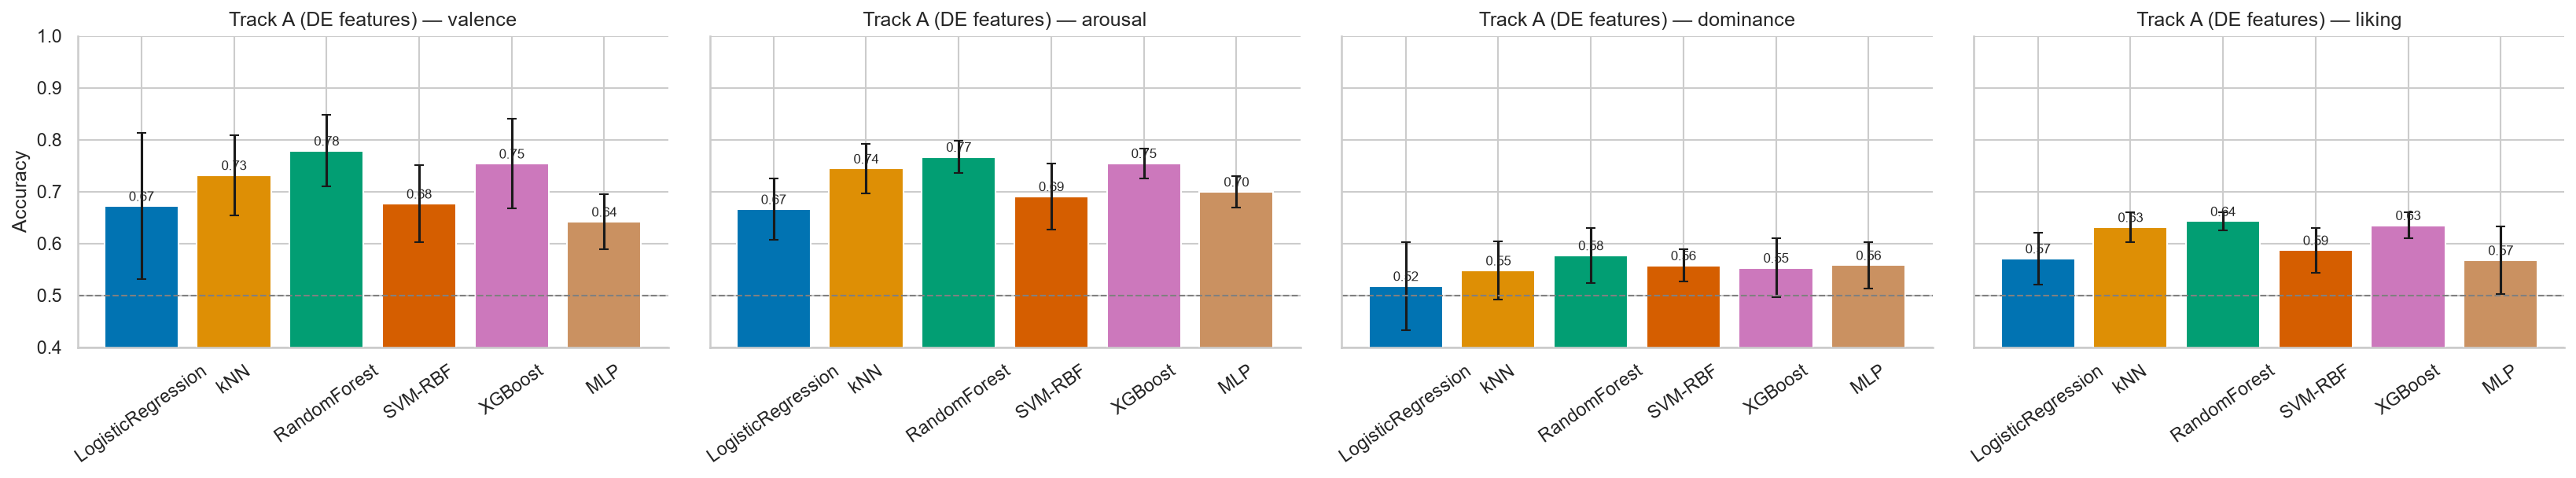
\includegraphics[width=0.85\textwidth]{track_a_accuracy.png}
\caption{Track A --- accuracy/F1/ROC-AUC for all six classical models across
all four tasks (5-fold GroupKFold).}
\label{fig:track-a-accuracy}
\end{figure}

\section{Section 6 -- Track B: Raw Windows $\to$ Deep Learning}
\label{sec:s6}

\subsection{6.1 Model architectures}
Four architectures, all implemented from scratch in PyTorch (also mirrored
in \texttt{scripts/dl\_models.py} for reuse by the companion scripts,
Chapter~\ref{ch:scripts}):
\begin{itemize}
  \item \textbf{EEGNet} (Lawhern et al.\ 2018, 2130 params): temporal conv
        $\to$ depthwise spatial conv $\to$ separable conv, purpose-built for
        EEG.
  \item \textbf{ShallowConvNet} (Schirrmeister et al.\ 2017, 54562 params):
        temporal conv $\to$ spatial conv $\to$ square/log-power nonlinearity,
        inspired by FBCSP-style band-power features.
  \item \textbf{CNN-LSTM} (82466 params): a spatial-temporal CNN front-end
        collapses the channel dimension; a bidirectional LSTM models the
        resulting temporal sequence.
  \item \textbf{TSception} (Ding et al.\ 2022, 8765 params): multi-scale
        temporal ``inception'' branches at three kernel sizes, fused with a
        global spatial conv and a hemisphere-asymmetry spatial conv (using
        DEAP's standard channel order) --- a simplified, faithful-in-spirit
        reimplementation, not a line-for-line port of the original codebase.
\end{itemize}

\subsection{6.2 Training loop}
\texttt{subject\_independent\_split} performs a nested
\texttt{GroupShuffleSplit}: 70/15/15 train/val/test by subject, so no
subject's data crosses a split boundary. \texttt{train\_torch\_model} trains
with \texttt{AdamW}, \texttt{ReduceLROnPlateau}, automatic mixed precision
(\texttt{torch.autocast} + \texttt{GradScaler}, active whenever CUDA is
available), early stopping on validation loss (patience 8, max 40 epochs),
and restores the best validation-loss checkpoint before final test
evaluation.

\subsection{6.3 Training all four models on all four tasks}
16 training runs (4 architectures $\times$ 4 tasks), single
train/val/test split, on the GPU. Table~\ref{tab:track-b-best} shows the
best model per task.

\begin{table}[h]
\centering
\caption{Track B --- best deep model per task (single subject-independent split)}
\label{tab:track-b-best}
\begin{tabular}{lllrrr}
\toprule
Task & Best model (by AUC) & Accuracy & F1 (macro) & ROC-AUC \\
\midrule
valence   & EEGNet     & 0.835 & 0.455 & 0.561 \\
arousal   & EEGNet     & 0.699 & 0.572 & 0.607 \\
dominance & TSception  & 0.589 & 0.414 & 0.475 \\
liking    & CNN-LSTM   & 0.599 & 0.384 & 0.497 \\
\bottomrule
\end{tabular}
\end{table}

Notably \textbf{dominance/EEGNet posts AUC 0.288} --- below chance, the
single worst result in either track, and an early instance of the
arousal/dominance instability pattern that recurs throughout
Sections~\ref{sec:s16}--\ref{sec:s17}.

\begin{figure}[H]
\centering
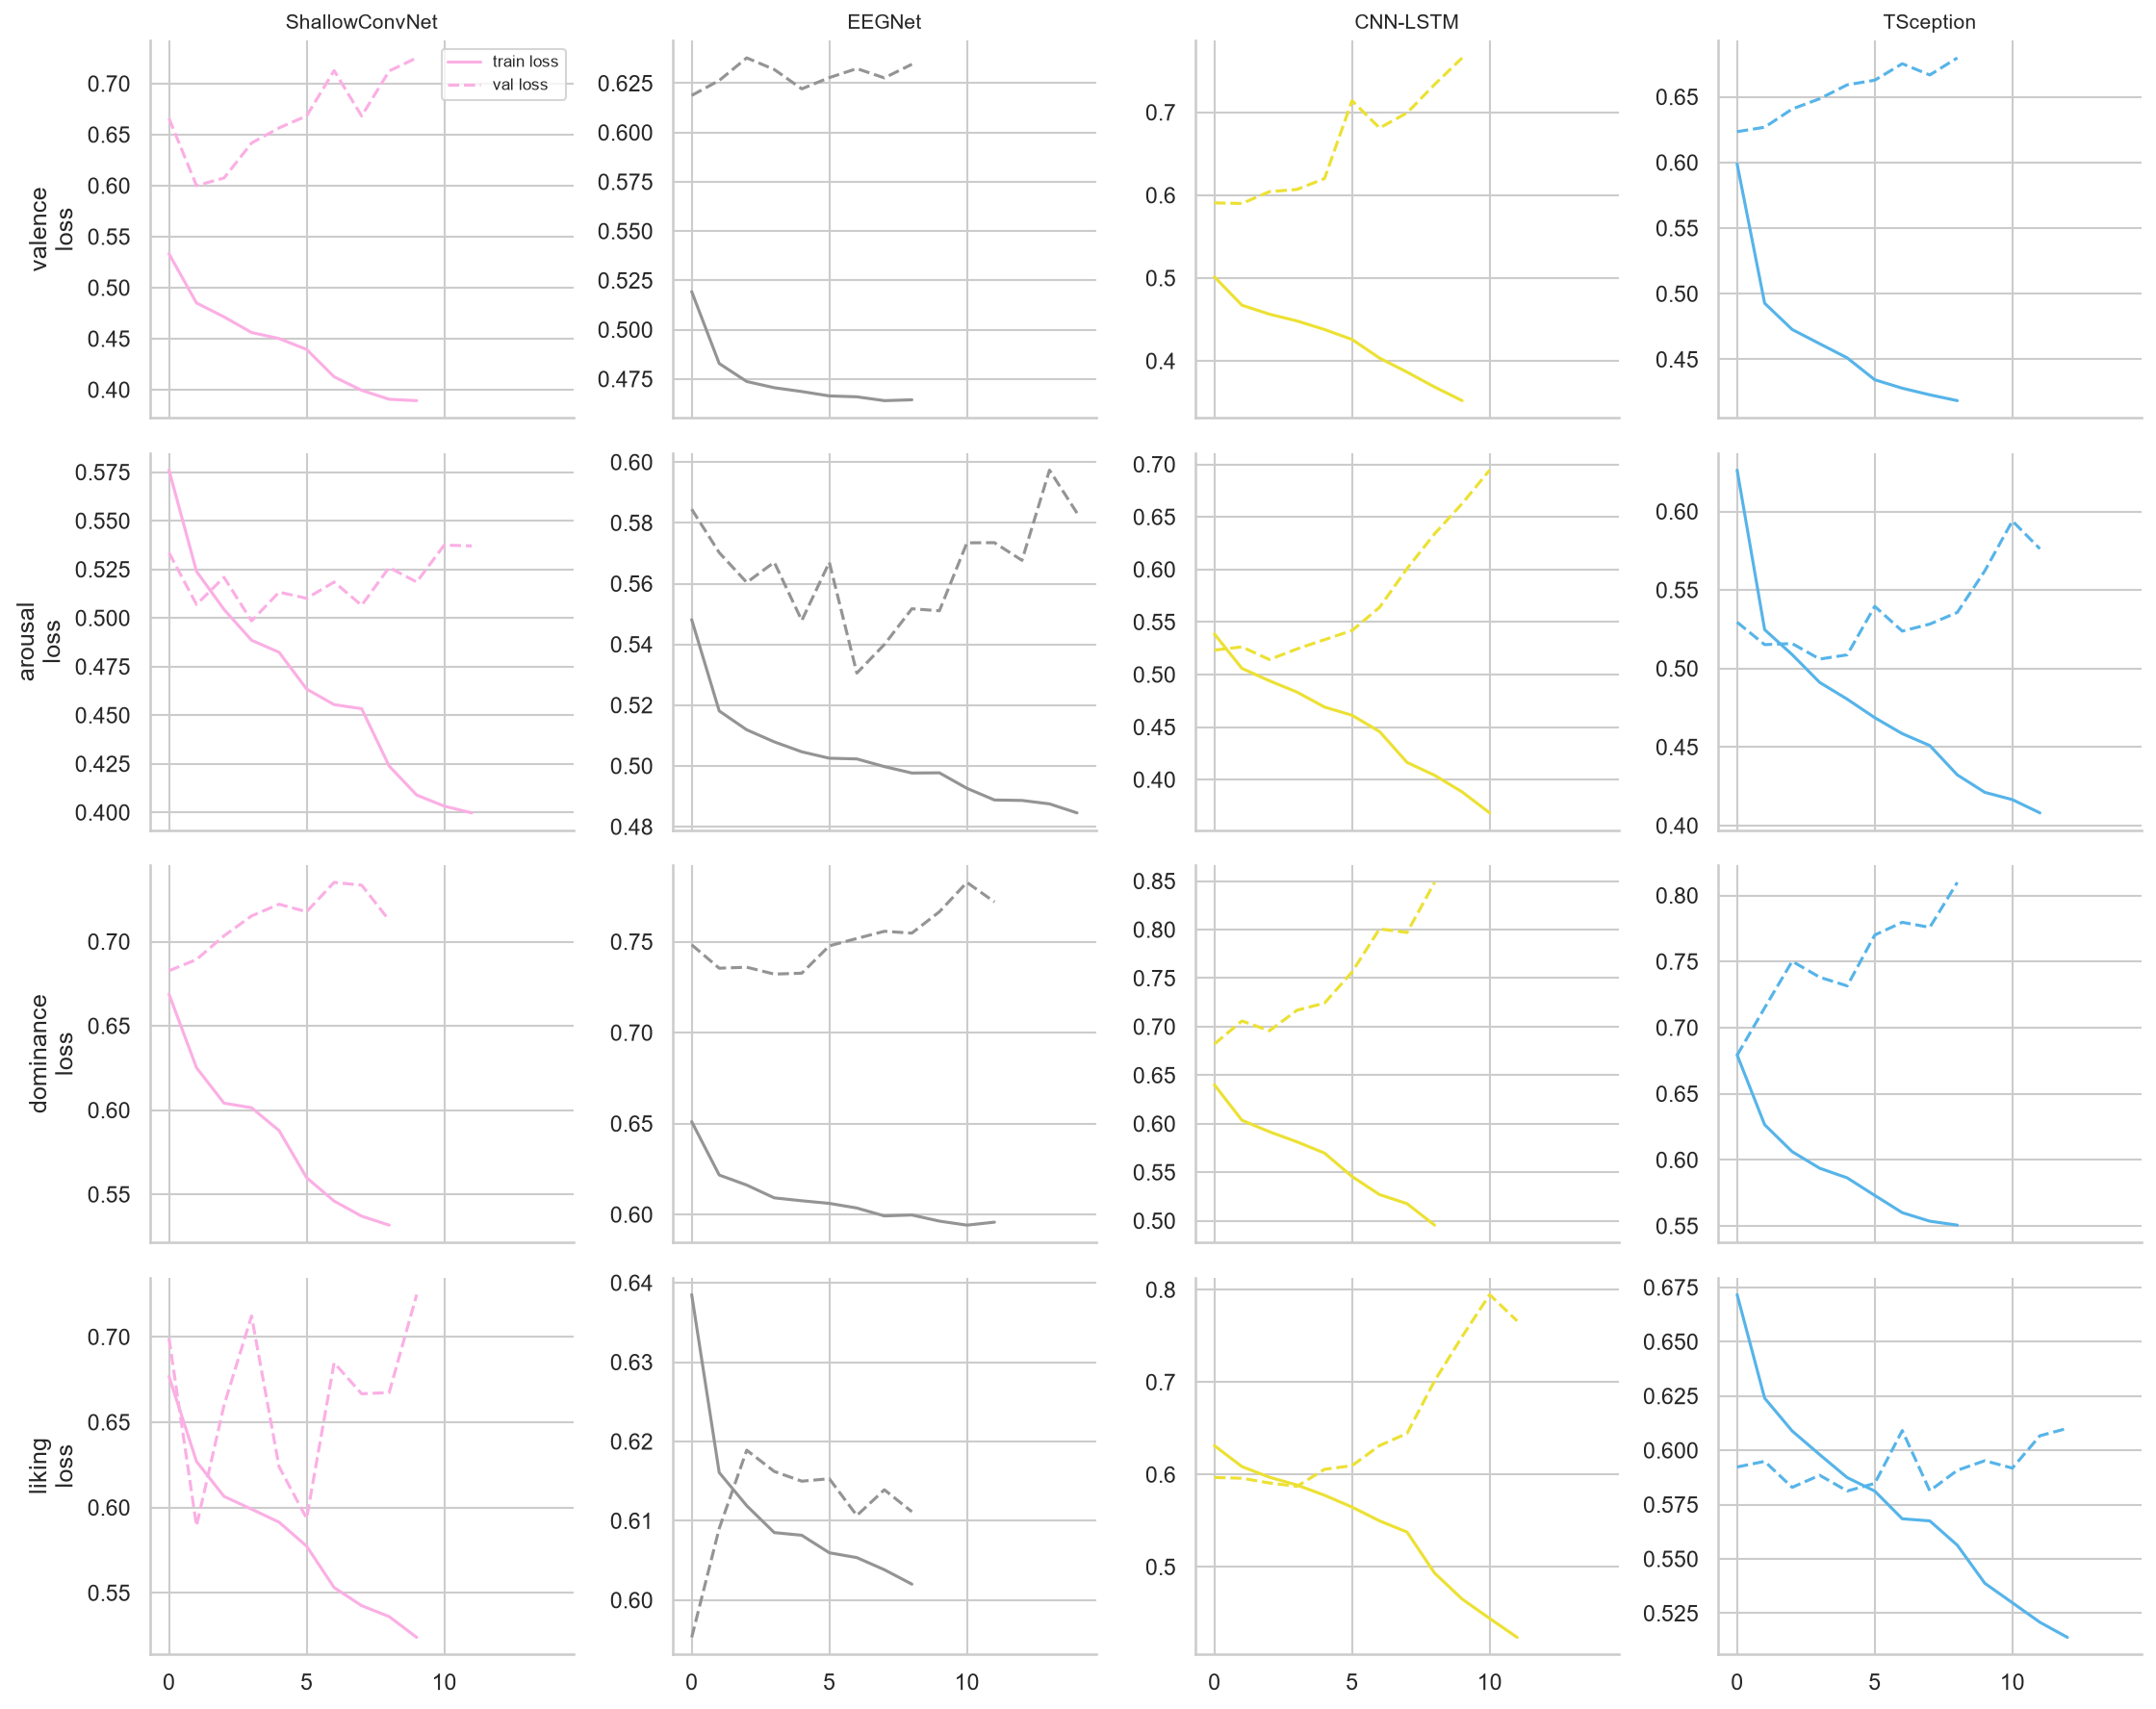
\includegraphics[width=0.9\textwidth]{track_b_training_curves.png}
\caption{Track B --- training/validation loss curves for all 16 runs
(4 architectures $\times$ 4 tasks), showing early-stopping behaviour under
the patience-8 schedule.}
\label{fig:track-b-training-curves}
\end{figure}

\section{Section 7 -- Combined Comparative Analysis}
Concatenates Track A and Track B results into a single 10-model table
(\texttt{results\_all}, saved to \texttt{combined\_results\_all.csv}),
plots accuracy/F1/AUC side by side across all 10 models $\times$ 4 tasks,
and plots confusion matrices for the best model per task.

\begin{figure}[H]
\centering
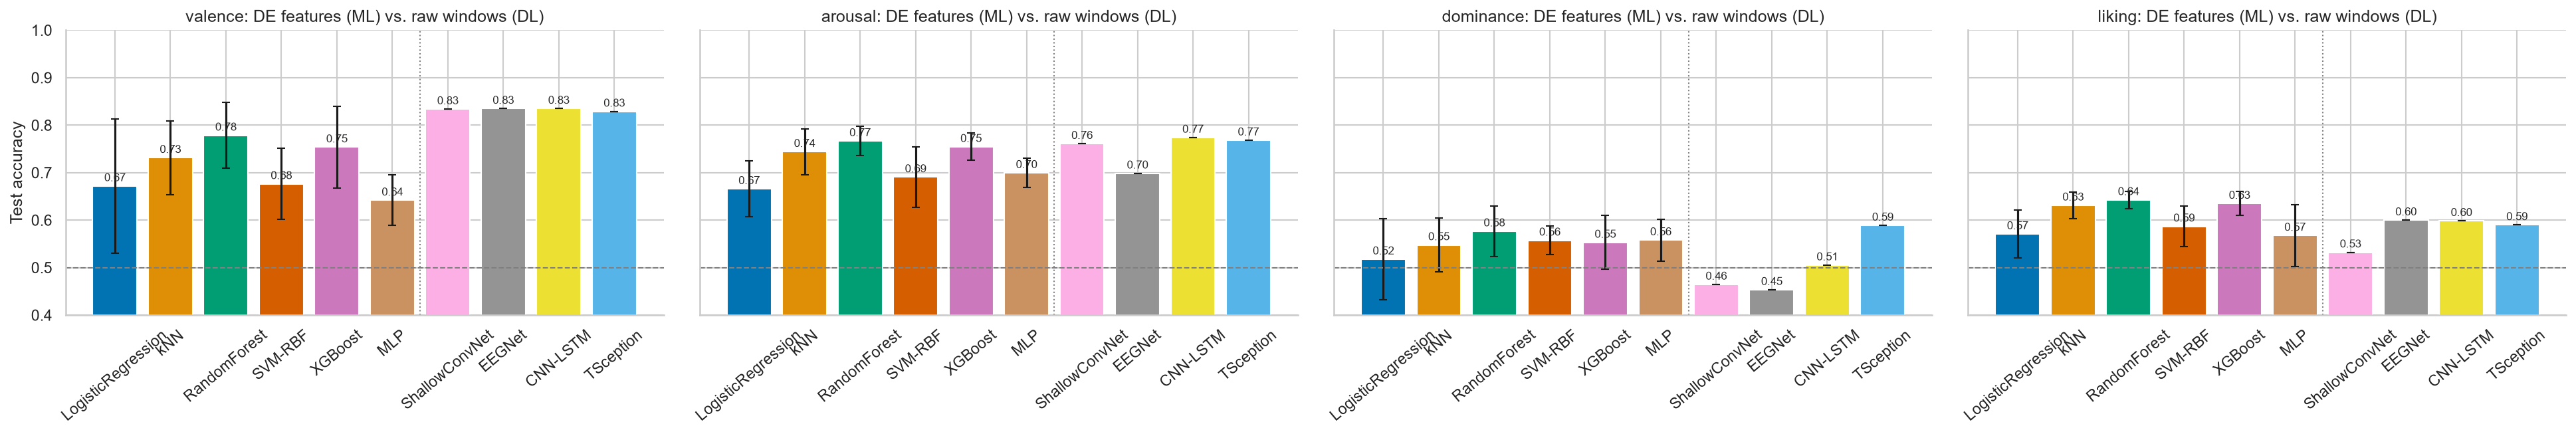
\includegraphics[width=0.9\textwidth]{combined_accuracy_comparison.png}
\caption{Combined accuracy/F1/ROC-AUC comparison across all 10 models
(6 classical + 4 deep) and all 4 tasks.}
\label{fig:combined-accuracy}
\end{figure}

\begin{figure}[H]
\centering
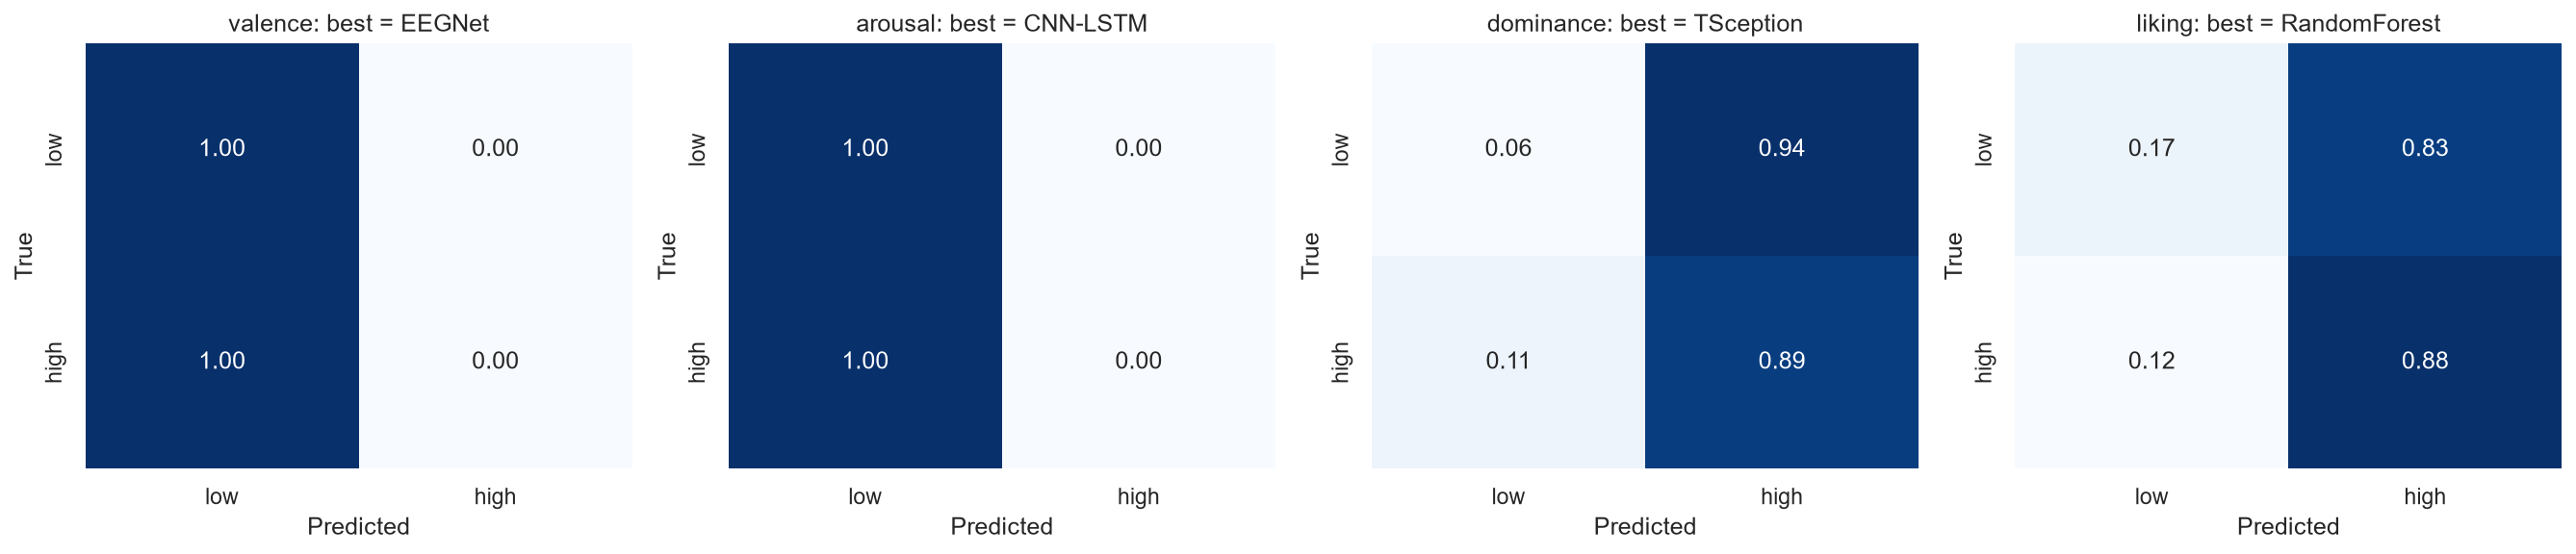
\includegraphics[width=0.85\textwidth]{confusion_matrices_best_models.png}
\caption{Confusion matrices for the best model per task (by ROC-AUC),
Tables~\ref{tab:track-a-best}/\ref{tab:track-b-best}.}
\label{fig:confusion-matrices}
\end{figure}

\section{Section 8 -- Discussion (initial)}
\label{sec:s8}
This section was originally written \emph{before} the notebook had been run
(a template: ``interpret the tables once the run completes''); it was
rewritten during this project against the real executed numbers above. Key
points:
\begin{itemize}
  \item \textbf{Neither track wins outright.} Track B edges out Track A on
        valence and arousal; Track A edges out Track B on dominance and
        liking. No model on either track clears $\sim0.61$ AUC on any task
        --- every one of the 10 models, on every one of the 4 tasks, sits in
        a narrow 0.45--0.61 band, barely-to-not-quite above chance. This is
        the first appearance of the pattern the rest of the notebook spends
        ten sections trying (and mostly failing) to explain away.
  \item \textbf{The imbalance artifact, quantified.} Valence is the most
        skewed task (79\% majority class), not liking as originally guessed.
        Track B's valence models hit 83.5\% accuracy at only $\sim$0.56 AUC
        --- both numbers sit within a couple of points of the 79\% majority
        baseline, the textbook signature of a classifier leaning on class
        imbalance rather than genuine signal.
  \item \textbf{Compute cost.} Track A's cheapest models (kNN, XGBoost,
        LogisticRegression) are 10--1000$\times$ cheaper per fit than any
        Track B model, and Track A's numbers are 5-fold cross-validated
        means, whereas Track B's are single-split point estimates
        ($\texttt{std}=0$ in the CSV means $n=1$, not zero variance ---
        Section~\ref{sec:s11} later adds repeats).
  \item \textbf{Subject independence is the hard setting}, and Section 13
        later quantifies exactly how much harder: this project's genuine
        subject-independent AUC ($\sim$0.45--0.56) sits far below the source
        MethodsX paper's own reported 0.97 ROC-AUC on the same dataset.
\end{itemize}

\section{Section 9 -- Richer Track A Features}
\label{sec:s9}
Three additional feature families are added to the 128-dim DE baseline (all
implemented in \texttt{scripts/rich\_features.py}, built for all 32 subjects
by \texttt{scripts/build\_extended\_features.py} into
\texttt{deap\_features\_ext\_v1.npz}, 19{,}200 windows $\times$ 295 features):
\begin{itemize}
  \item \textbf{Hjorth parameters} (activity, mobility, complexity) --- 96
        features (3 $\times$ 32 channels), classic time-domain complexity
        descriptors DE alone misses.
  \item \textbf{Frontal/hemispheric alpha asymmetry (FAA)} --- 14 features,
        $\text{alpha}_{\text{right}} - \text{alpha}_{\text{left}}$ per
        electrode pair --- the classic Davidson-style valence marker.
  \item \textbf{Connectivity (PLV + coherence)} --- 57 features across 19
        curated channel pairs: phase-locking value in alpha and beta bands
        (38 features) plus alpha-band magnitude-squared coherence (19
        features), computed via a Hilbert-transform / Welch-style pipeline
        implemented from scratch in \texttt{rich\_features.py}.
\end{itemize}

\subsection{Feature-set ablation (\texttt{track\_a\_ablation.py})}
6 feature-set combinations $\times$ 3 representative models
(LogisticRegression, RandomForest, XGBoost) $\times$ 4 tasks $\times$ 5-fold
\texttt{GroupKFold} = 360 fits. \textbf{Real result}: mean AUC across all six
feature sets ranges only from 0.478 (DE+Hjorth) to 0.494
(DE+Connectivity) --- every configuration stays in the 0.42--0.56 range
observed in Section~\ref{sec:s5}/\ref{sec:s6}. None of the three additions
move AUC meaningfully off chance for any task. The ``Full'' set is carried
forward to Section~\ref{sec:s10} as the most complete configuration, not
because the ablation crowned it a clear winner.

\begin{table}[H]
\centering
\caption{Feature-set ablation --- mean ROC-AUC across 3 models $\times$ 4
tasks (12 fits) per feature set}
\label{tab:ablation}
\begin{tabular}{lrr}
\toprule
Feature set & \#Features & Mean ROC-AUC \\
\midrule
DE only                       & 128 & 0.479 \\
DE + Hjorth                   & 224 & 0.478 \\
DE + FAA                      & 142 & 0.483 \\
DE + Connectivity             & 185 & 0.494 \\
DE + Hjorth + FAA             & 238 & 0.479 \\
Full (DE+Hjorth+FAA+Conn)     & 295 & 0.483 \\
\bottomrule
\end{tabular}
\end{table}

\begin{figure}[H]
\centering
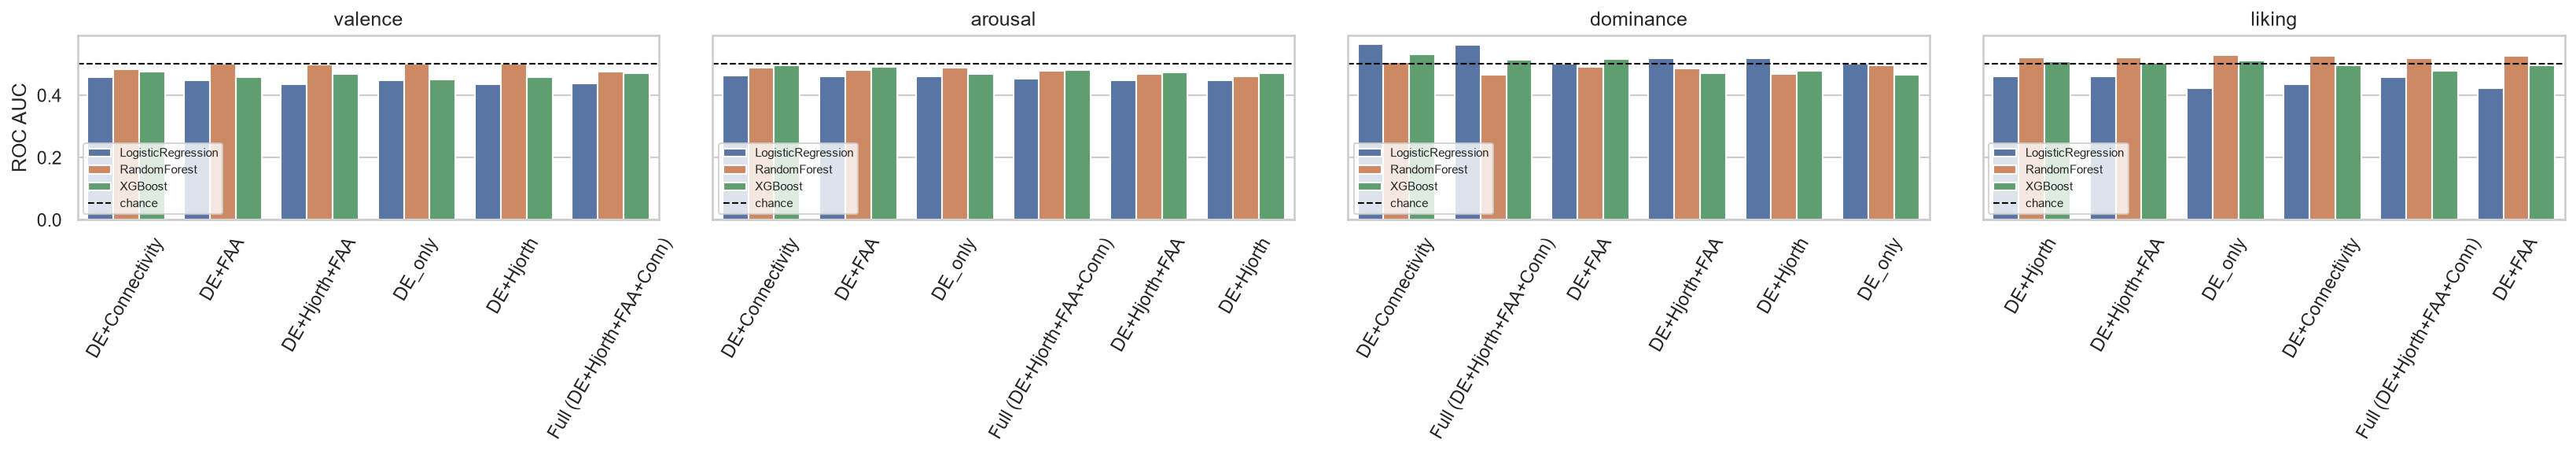
\includegraphics[width=0.85\textwidth]{track_a_ablation_auc.png}
\caption{Feature-set ablation --- ROC-AUC by feature set, model, and task.}
\label{fig:ablation}
\end{figure}

\section{Section 10 -- Repeated \& Nested GroupKFold}
\label{sec:s10}
Two upgrades, run via \texttt{track\_a\_repeated\_nested\_cv.py}:
\begin{enumerate}
  \item \textbf{Repeated GroupKFold} (5 repeats $\times$ 5 folds = 25 folds
        per model/task), giving every AUC a real 95\% confidence interval.
        Because \texttt{sklearn} has no \texttt{RepeatedGroupKFold}, each
        repeat randomly relabels the 32 subject IDs before calling
        \texttt{GroupKFold(5)} (its greedy fold assignment is sensitive to
        the sorted order of group labels, so relabeling yields a genuinely
        different subject-to-fold partition each repeat).
  \item \textbf{Nested CV} for XGBoost and RandomForest: outer
        \texttt{GroupKFold(5)}, inner \texttt{GroupKFold(3)} via
        \texttt{RandomizedSearchCV} (8 draws), checking whether the fixed,
        hand-picked hyperparameters used everywhere else were leaving
        accuracy on the table.
\end{enumerate}
\textbf{Real result}: of 24 model/task 95\% AUC confidence intervals, 15
contain 0.5 (chance). The 9 that do \emph{not} skew mostly toward dominance
and liking (e.g.\ dominance/LogisticRegression: 0.571, CI [0.546, 0.597];
liking/kNN: 0.532, CI [0.518, 0.546]). Nested hyperparameter search does not
close the gap either --- e.g.\ dominance/XGBoost tuned AUC 0.494 vs.\ 0.517
fixed-hyperparameter (Section~\ref{sec:s9}), essentially unchanged. Combined,
these rule out ``the fixed hyperparameters were the bottleneck'' as an
explanation.

\begin{figure}[H]
\centering
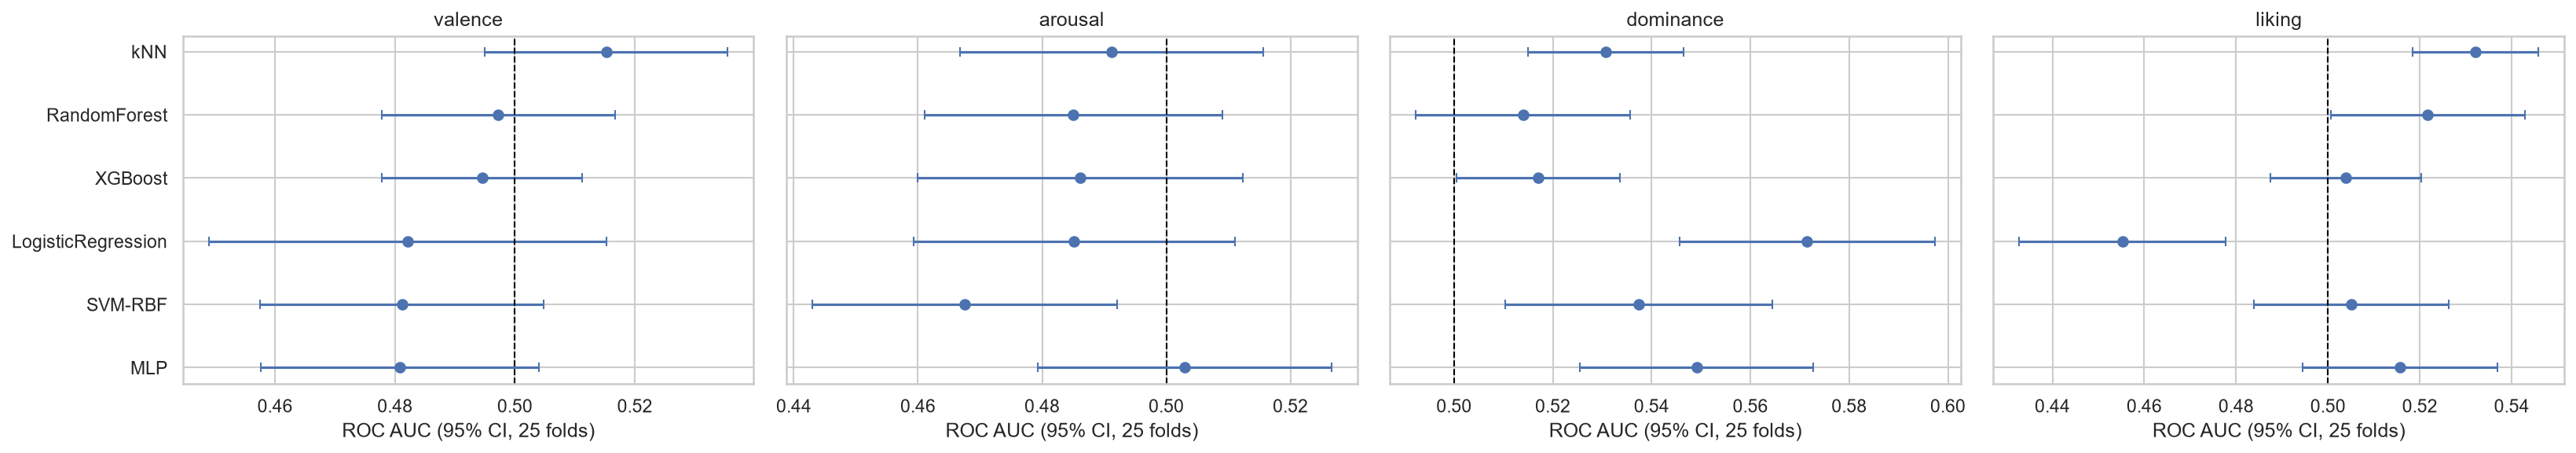
\includegraphics[width=0.9\textwidth]{track_a_repeated_cv_auc_ci.png}
\caption{Repeated GroupKFold (5$\times$5=25 folds) --- ROC-AUC with 95\%
confidence intervals per model/task; 15/24 intervals contain chance (0.5).}
\label{fig:repeated-cv}
\end{figure}

\section{Section 11 -- 50\% Overlapping Windows + Repeated Track B Splits}
\label{sec:s11}
\texttt{scripts/build\_overlap\_windows.py} builds a second raw-window cache
with stride $=256$ samples (2\,s, i.e.\ 50\% overlap) instead of 512,
giving 29 windows/trial instead of 15 (37{,}120 windows total). A leakage
caveat is documented explicitly: overlapping windows share up to 50\% of
their raw samples and are \emph{not} independent observations --- subject
grouping prevents cross-subject leakage but not this within-subject
correlation. \texttt{scripts/track\_b\_repeated.py} then runs 5 repeated
70/15/15 subject-independent splits, both window variants, all 4
architectures, all 4 tasks (160 training runs, $\sim$87 minutes on the
project's RTX 3070 Ti). \textbf{Real result}: mean AUC across all
model/task combinations is 0.483 (non-overlap) vs.\ 0.498 (overlap50) ---
deltas are small and inconsistent in sign, consistent with the
non-independence caveat: more correlated windows is not the same as more
information.

\begin{figure}[H]
\centering
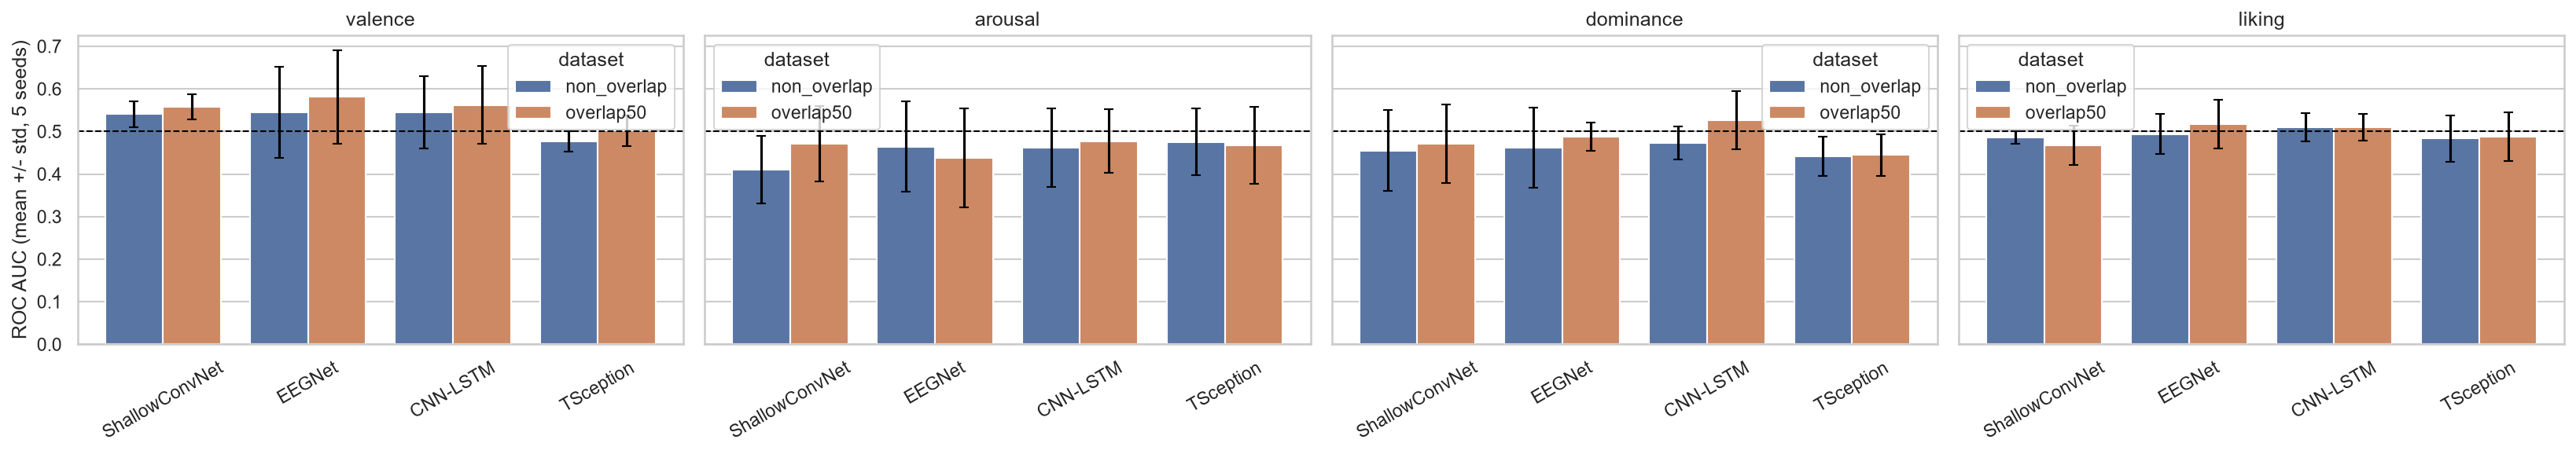
\includegraphics[width=0.85\textwidth]{track_b_overlap_vs_nonoverlap_auc.png}
\caption{Repeated Track B splits --- ROC-AUC, non-overlapping vs.\ 50\%-overlap
windows, across 4 architectures $\times$ 4 tasks.}
\label{fig:overlap}
\end{figure}

\section{Section 12 -- Cross-Corpus Validation (SEED-IV)}
\label{sec:s12}
\subsection{Why SEED-IV, not original SEED}
Original SEED requires a signed BCMI data-use agreement; DREAMER and AMIGOS
require similar gated requests. SEED-IV, a related 4-class dataset from the
same lab, is mirrored on Kaggle with no agreement required, so it is the one
target corpus in this pipeline that could actually be obtained and run.

\subsection{Pipeline (\texttt{scripts/cross\_corpus/})}
\label{sec:seed-iv-adapter}
\begin{itemize}
  \item \texttt{base.py}: dataset-agnostic infrastructure --- channel-name
        intersection between DEAP and a target montage
        (\texttt{intersect\_channels}), resampling
        (\texttt{resample\_signal}, polyphase via
        \texttt{scipy.signal.resample\_poly}), generic band-DE extraction
        restricted to the common channel subset
        (\texttt{compute\_de\_features\_generic},
        \texttt{extract\_common\_channel\_de}), rebuilding DEAP's own DE
        features on that same restricted/reordered channel set
        (\texttt{build\_deap\_common\_channel\_dataset}, so the DEAP-side
        model is retrained fairly rather than fed a mismatched feature
        vector), and zero-shot evaluation with per-subject breakdown
        (\texttt{evaluate\_zero\_shot}).
  \item \texttt{seed\_adapter.py} (\texttt{SeedIVAdapter}): loads SEED-IV's
        \texttt{eeg\_raw\_data/\{1,2,3\}/*.mat} session files (62 channels,
        200\,Hz), resolves the channel-order file defensively across several
        candidate filenames (the Kaggle mirror ships \texttt{Channel
        Order.xlsx}, not the hyphenated \texttt{channel-order.xlsx}
        originally assumed), and resolves per-session labels defensively:
        it first tries to load a real label file, and --- since the actual
        download ships no separate label \texttt{.mat} file, only prose in
        \texttt{ReadMe.txt} --- falls back to the label sequence published
        in the SEED-IV paper with a loud warning. This fallback was
        cross-checked byte-for-byte against the real \texttt{ReadMe.txt} and
        matches exactly. \texttt{binarize\_label} maps SEED-IV's 4 classes
        onto a valence-like binary task: happy $=1$ (positive), sad/fear
        $=0$ (negative), neutral dropped.
  \item \texttt{run\_cross\_corpus.py}: orchestrates (1) a within-DEAP
        \texttt{GroupKFold} baseline on the 32 common channels shared with
        SEED-IV, (2) DEAP$\to$SEED-IV zero-shot transfer (train on all of
        DEAP, never see SEED-IV), (3) a SEED-IV-only LOSO baseline (32
        subjects $\to$ 15 folds, one per SEED-IV subject).
\end{itemize}

\subsection{Real result}
\begin{table}[h]
\centering
\caption{Cross-corpus validation --- DE + XGBoost, 32 common channels}
\label{tab:cross-corpus}
\begin{tabular}{lrrr}
\toprule
Setting & Accuracy & ROC-AUC & Notes \\
\midrule
Within-DEAP GroupKFold      & 0.756 & \textbf{0.452} & below chance point estimate \\
DEAP$\to$SEED-IV zero-shot  & 0.709 & \textbf{0.517} & marginally above chance \\
SEED-IV-only LOSO           & 0.709 & \textbf{0.673} & 12/15 subjects $>$0.55 AUC \\
\bottomrule
\end{tabular}
\end{table}
This reframes the question Section~12 originally set out to answer. DEAP's
own within-corpus signal is \emph{not} inflated relative to genuine
cross-corpus transfer --- it is the weakest of the three settings. The
\emph{identical} pipeline reaches a real, moderate AUC of 0.673 on SEED-IV
under a directly comparable protocol, ruling out ``subject-independent EEG
emotion decoding is just hard everywhere'' as an explanation. The near-chance
ceiling documented throughout this notebook is better attributed to
something specific to DEAP (its 1--9 self-report threshold, its stimulus
set, or its labelling protocol) than to the modelling task in general.
Caveats: SEED-IV's binary construct (happy vs.\ sad/fear) is not the same as
DEAP's continuous valence threshold; the two corpora differ in session count
and per-trial duration; and restricting to 32 common channels discards
SEED-IV's denser 62-channel coverage.

\begin{figure}[H]
\centering
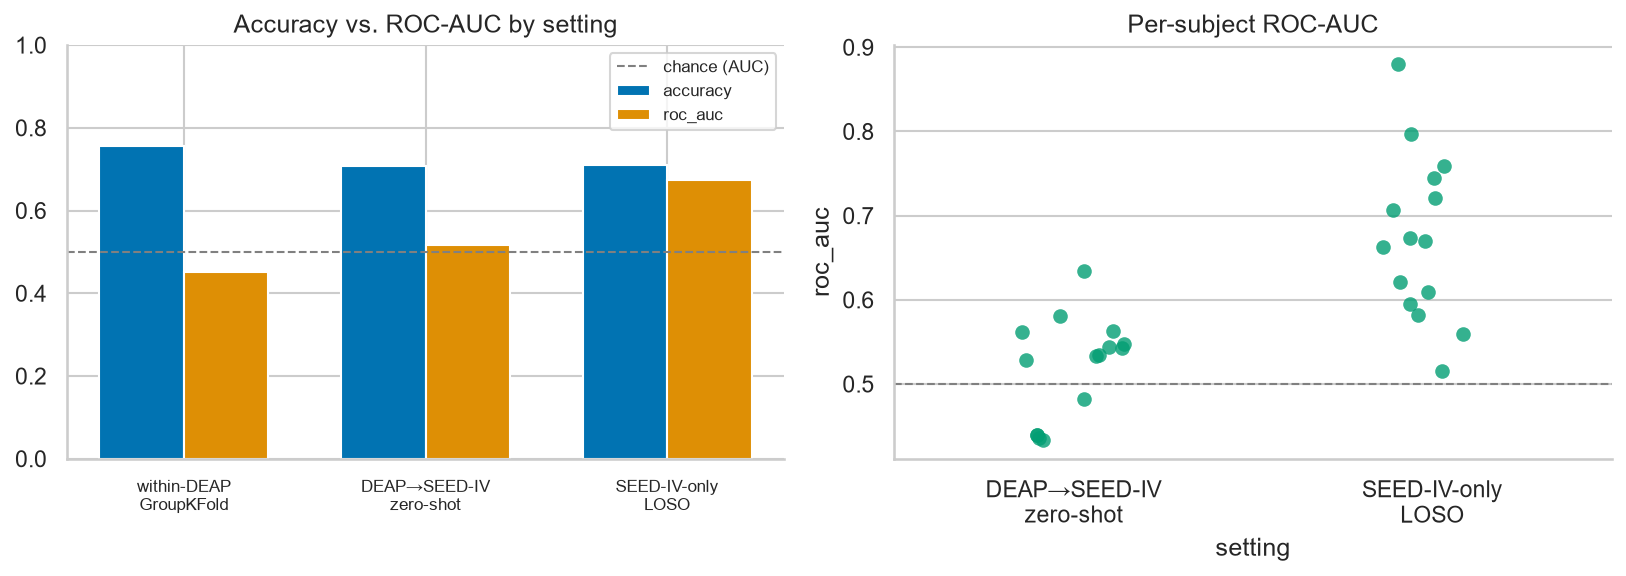
\includegraphics[width=0.85\textwidth]{cross_corpus_deap_seediv.png}
\caption{Cross-corpus validation --- ROC-AUC across the three settings of
Table~\ref{tab:cross-corpus} (within-DEAP, DEAP$\to$SEED-IV zero-shot,
SEED-IV-only LOSO).}
\label{fig:cross-corpus}
\end{figure}

\section{Section 13 -- Updated Overall Discussion}
\label{sec:s13}
Synthesises Sections 9--12. Central claims: (1) AUC hovers within noise of
chance almost everywhere, and this is the single most important finding;
(2) none of richer features, repeated/nested CV, or window overlap ``fixed''
the ceiling, which is itself informative --- each rules out a specific,
plausible cause rather than being a failed implementation; (3) the
cross-corpus result overturns the section's own original speculation (``DEAP
signal is simply weak $\Rightarrow$ transfer will be weak too''), reframing
the finding as DEAP-specific rather than universal; (4) the practical
recommendation for any paper drawn from this work is to lead with the
leaky-split contrast: this project's $\sim$0.45--0.56 AUC under genuine
\texttt{GroupKFold} vs.\ the source MethodsX paper's reported 0.97 ROC-AUC
on the same dataset and a similar feature/classifier combination.

\section{Section 14 -- Label-Cleanup Ablation}
\label{sec:s14}
\texttt{scripts/track\_a\_label\_cleanup.py} tests three ways of turning
continuous ratings into binary labels (Full feature set, 3 models, 4 tasks,
\texttt{GroupKFold(5)}):
\begin{itemize}
  \item \textbf{raw\_threshold} (baseline): fixed cutoff at 5.0.
  \item \textbf{per\_subject\_z}: z-score each subject's own 40 ratings
        before thresholding at 0, correcting for individual anchoring bias.
  \item \textbf{drop\_middle}: keep only ratings $\le3$ or $\ge6$, discarding
        the ambiguous middle.
\end{itemize}
\textbf{Real result}: mean AUC is 0.483 (raw\_threshold), 0.514
(per\_subject\_z), 0.487 (drop\_middle). \texttt{per\_subject\_z} rebalances
classes substantially (valence goes from 21.0\% to 47.3\% high) and gives
the largest AUC bump, but the gain is modest and the class-balance shift
means its accuracy numbers must \emph{not} be compared directly to the
baseline's. Neither alternative reliably beats the baseline enough to rule
in ``the fixed-threshold label was the bottleneck.''

\begin{table}[H]
\centering
\caption{Label-cleanup ablation --- mean ROC-AUC across 3 models $\times$
4 tasks per label variant}
\label{tab:label-cleanup}
\begin{tabular}{lr}
\toprule
Label variant & Mean ROC-AUC \\
\midrule
raw\_threshold (baseline) & 0.483 \\
per\_subject\_z           & 0.514 \\
drop\_middle               & 0.487 \\
\bottomrule
\end{tabular}
\end{table}

\begin{figure}[H]
\centering
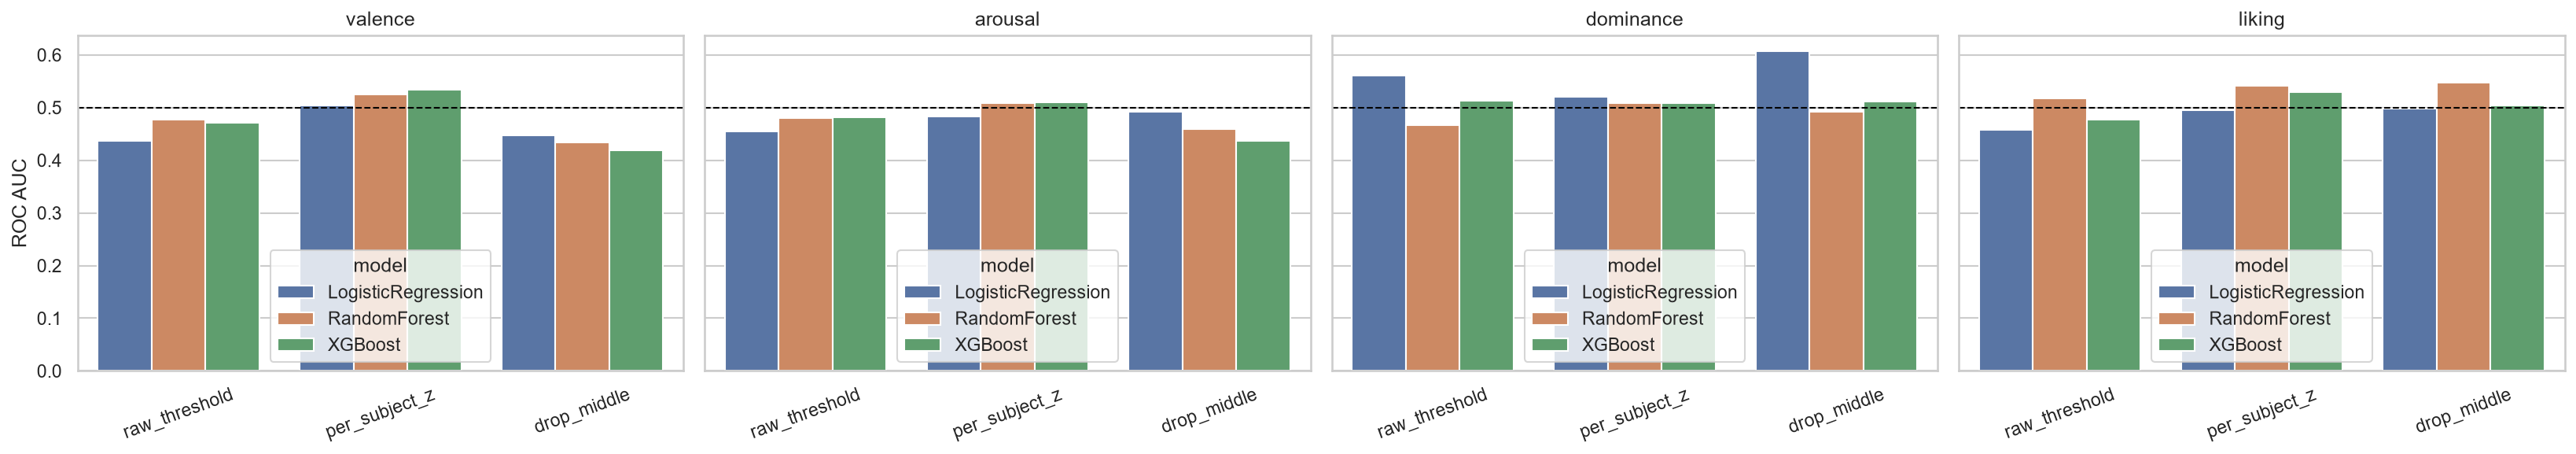
\includegraphics[width=0.85\textwidth]{track_a_label_cleanup_auc.png}
\caption{Label-cleanup ablation --- ROC-AUC by label variant, model, and
task.}
\label{fig:label-cleanup}
\end{figure}

\section{Section 15 -- Per-Subject Calibration (Personalisation)}
\label{sec:s15}
\texttt{scripts/track\_a\_calibration\_loso.py} runs a true 32-fold
Leave-One-Subject-Out with XGBoost (cheap enough to make full LOSO
tractable, $\sim$13\,s/subject). For each held-out subject: train a base
model on the other 31 subjects; split the held-out subject's 40 trials
80/20 into eval/calibration sets (by trial, so a trial's 15 windows never
cross the split); score the base model zero-shot on the eval set; then
warm-start $\sim$40 extra boosted trees on the 8-trial calibration set only,
and re-score on the identical eval set. Subjects whose calibration set is
single-class (13 across all 4 tasks) are skipped for the calibrated arm and
reported as such. \textbf{Real result}: mean zero-shot AUC is $\sim$0.50--0.51
across all four tasks; mean calibrated AUC rises to 0.577 (arousal), 0.519
(dominance), 0.539 (liking), 0.537 (valence) --- a real, if modest, positive
shift with a small amount of the target subject's own data, suggesting the
ceiling is not purely a between-subject-variability problem that a little
calibration data cannot touch, though 8 trials and 40 trees is a small
intervention.

\begin{figure}[H]
\centering
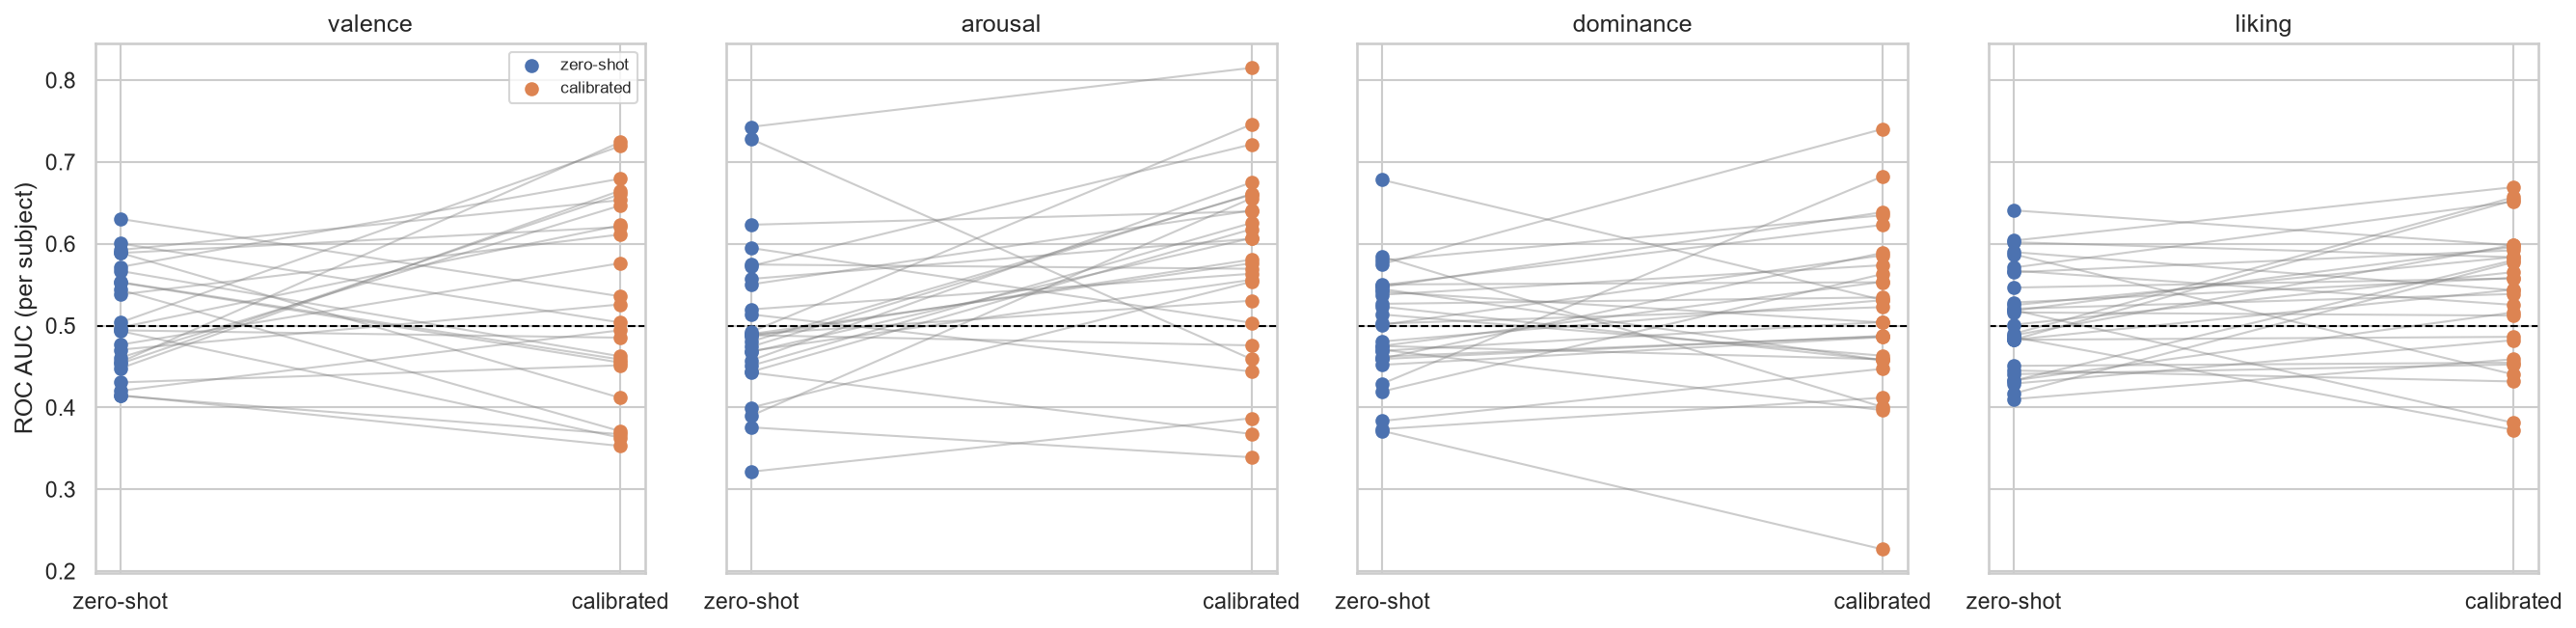
\includegraphics[width=0.9\textwidth]{track_a_calibration_per_subject.png}
\caption{Per-subject LOSO calibration --- zero-shot vs.\ calibrated ROC-AUC
for each of the 32 held-out subjects, per task.}
\label{fig:calibration}
\end{figure}

\section{Section 16 -- Literature-Driven Interventions}
\label{sec:s16}
31 papers in \texttt{papers\_EEG/} were assembled and reviewed (see
Chapter~\ref{ch:literature}), yielding three untried interventions.

\subsection{16.1 Permutation significance test}
\texttt{track\_a\_significance\_test.py} shuffles labels globally (preserving
\texttt{GroupKFold} fold structure), reruns the exact Full-feature-set
\texttt{GroupKFold(5)} pipeline with LogisticRegression (a fast, documented
proxy), and repeats 300 times per task to build an empirical null AUC
distribution;
$p = \frac{1 + \#\{\text{null} \ge \text{observed}\}}{n_{\text{perm}}+1}$.
\textbf{Real result}: for valence, arousal, and liking, observed AUC is
\emph{not} just close to the null, it is statistically indistinguishable
from it ($p=1.0$ for all three), and sits slightly \emph{below} the null
mean (e.g.\ valence: observed 0.437 vs.\ null $0.501\pm0.005$, $z=-12.0$).
\textbf{Dominance is the one exception}: observed 0.561 vs.\ null
$0.500\pm0.005$, $z=+12.3$, $p=0.0033$ --- genuinely significant, but still a
small effect.

\begin{table}[H]
\centering
\caption{Permutation significance test (300 shuffles per task, LogisticRegression proxy)}
\label{tab:significance}
\begin{tabular}{lrrrr}
\toprule
Task & Observed AUC & Null mean $\pm$ std & $z$ & $p$ \\
\midrule
valence   & 0.437 & $0.501\pm0.005$ & $-12.00$ & 1.0000 \\
arousal   & 0.454 & $0.500\pm0.005$ & $-8.30$  & 1.0000 \\
dominance & 0.561 & $0.500\pm0.005$ & $+12.28$ & 0.0033 \\
liking    & 0.458 & $0.500\pm0.005$ & $-8.27$  & 1.0000 \\
\bottomrule
\end{tabular}
\end{table}

\begin{figure}[H]
\centering
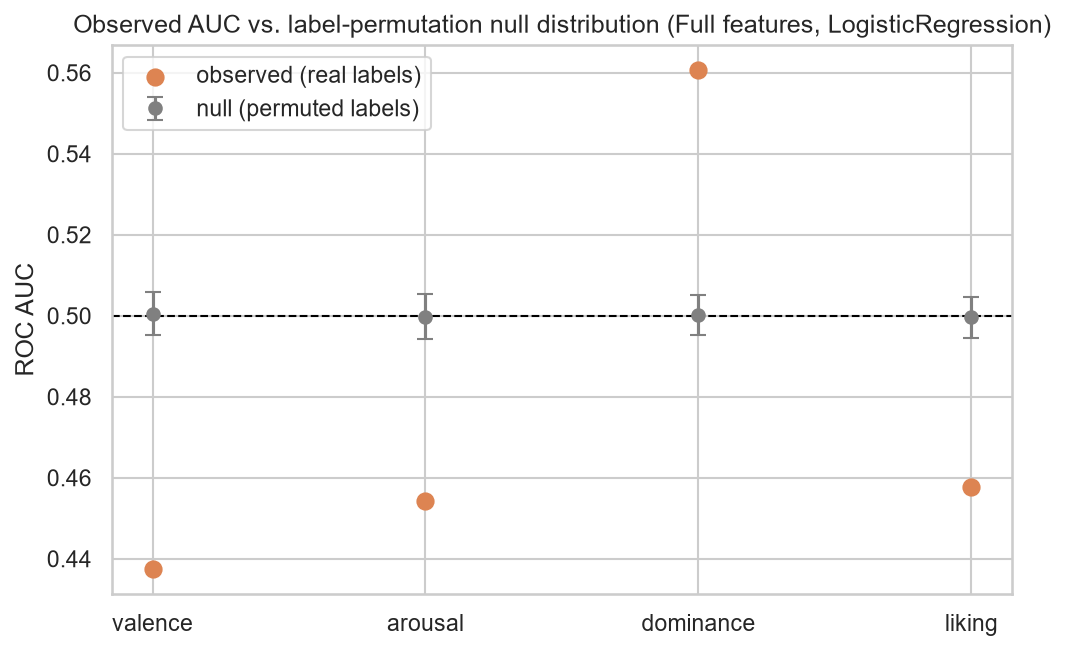
\includegraphics[width=0.85\textwidth]{track_a_significance_test.png}
\caption{Permutation null AUC distributions vs.\ observed AUC, per task.}
\label{fig:significance}
\end{figure}

\subsection{16.2 CORAL feature alignment}
\texttt{track\_a\_domain\_alignment.py} implements CORAL (Sun \& Saenko
2016): per \texttt{GroupKFold} fold, whiten the training fold's features by
their own covariance and recolour by the (unlabelled) test fold's
covariance, via eigendecomposition-based matrix square roots
($C^{-1/2}$, $C^{1/2}$) with a ridge for numerical stability. \textbf{Real
result}: mean AUC delta across 12 task/model combinations is $+0.0059$ (8/12
improved, 4/12 worse) --- small and inconsistent in sign.

\begin{table}[H]
\centering
\caption{CORAL alignment --- mean ROC-AUC across 3 models per task}
\label{tab:coral}
\begin{tabular}{lrrr}
\toprule
Task & No alignment & CORAL & $\Delta$ \\
\midrule
valence   & 0.462 & 0.478 & $+0.016$ \\
arousal   & 0.472 & 0.476 & $+0.004$ \\
dominance & 0.514 & 0.521 & $+0.008$ \\
liking    & 0.484 & 0.480 & $-0.004$ \\
\bottomrule
\end{tabular}
\end{table}

\begin{figure}[H]
\centering
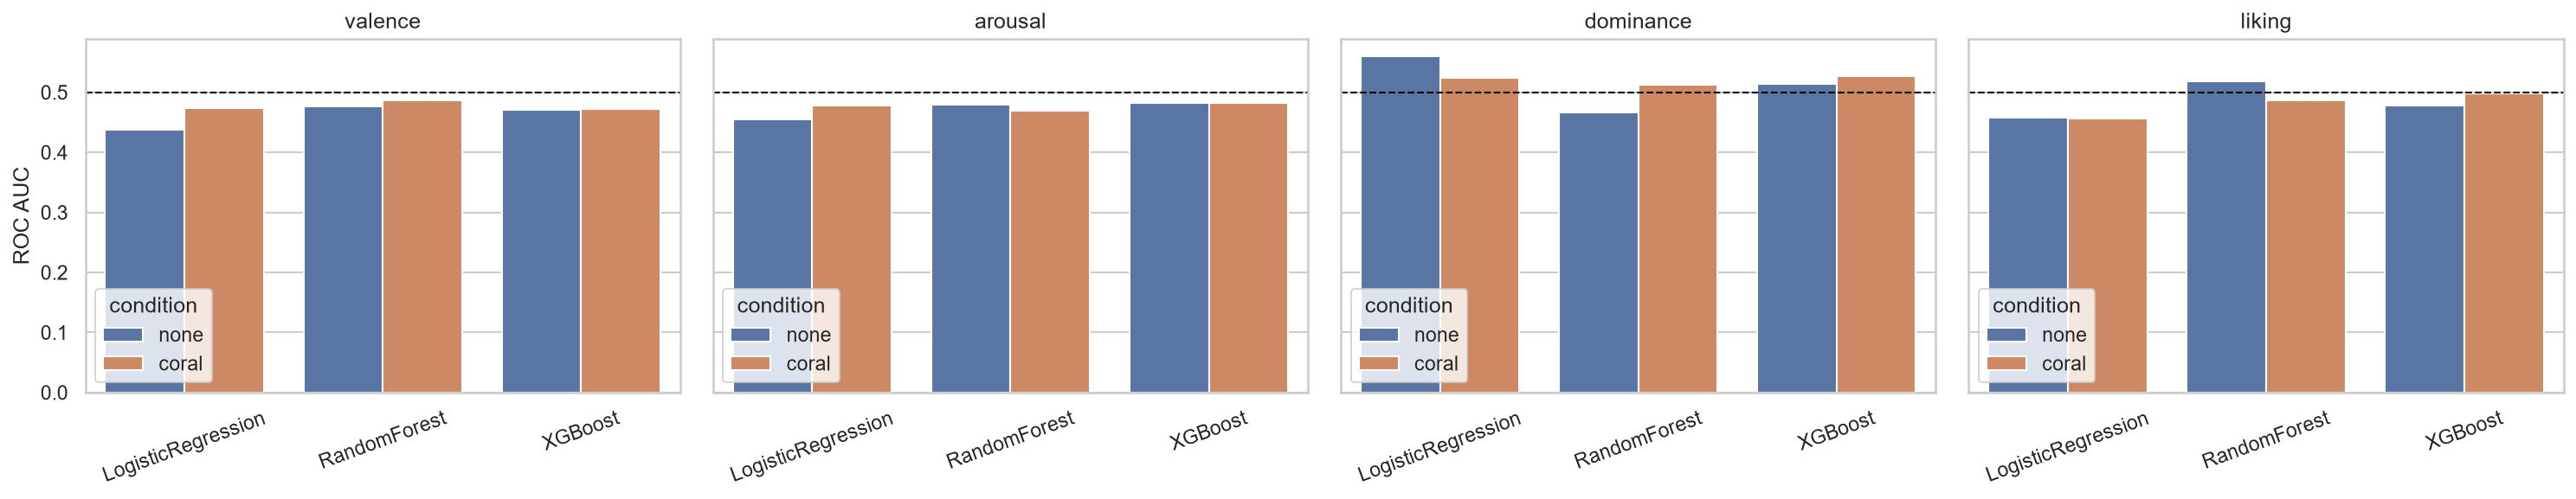
\includegraphics[width=0.85\textwidth]{track_a_domain_alignment_auc.png}
\caption{CORAL alignment --- ROC-AUC before/after, by model and task.}
\label{fig:coral}
\end{figure}

\subsection{16.3 Subject-adversarial (DANN) training}
\texttt{track\_b\_domain\_adversarial.py} adds a gradient-reversal-layer
(GRL) domain classifier to EEGNet, trained to predict the training-fold
subject's identity; the GRL reverses that gradient before it reaches the
shared encoder (standard Ganin \& Lempitsky 2016 progressive-$\lambda$
schedule, $\lambda_p = \tfrac{2}{1+e^{-10p}}-1$). \textbf{Real result}: a
mixed, task-dependent outcome. Valence AUC $0.474\to0.513$ ($+0.039$) and
liking AUC $0.467\to0.517$ ($+0.050$) improved; arousal AUC
$0.616\to0.400$ ($-0.216$) and dominance AUC $0.552\to0.403$ ($-0.149$)
collapsed, with precision/recall pinned near 0.50 --- the classifier
collapsing toward one class, not a milder generic drop. This matches a
documented UDA failure pattern (``over-aggressive alignment collapsing class
structure'') from the PRISMA review in the literature corpus.

\begin{table}[H]
\centering
\caption{Subject-adversarial (DANN) training --- ROC-AUC, EEGNet, single split}
\label{tab:dann}
\begin{tabular}{lrrr}
\toprule
Task & Baseline & DANN & $\Delta$ \\
\midrule
valence   & 0.474 & 0.513 & $+0.039$ \\
arousal   & 0.616 & 0.400 & $-0.216$ \\
dominance & 0.552 & 0.403 & $-0.149$ \\
liking    & 0.467 & 0.517 & $+0.050$ \\
\bottomrule
\end{tabular}
\end{table}

\begin{figure}[H]
\centering
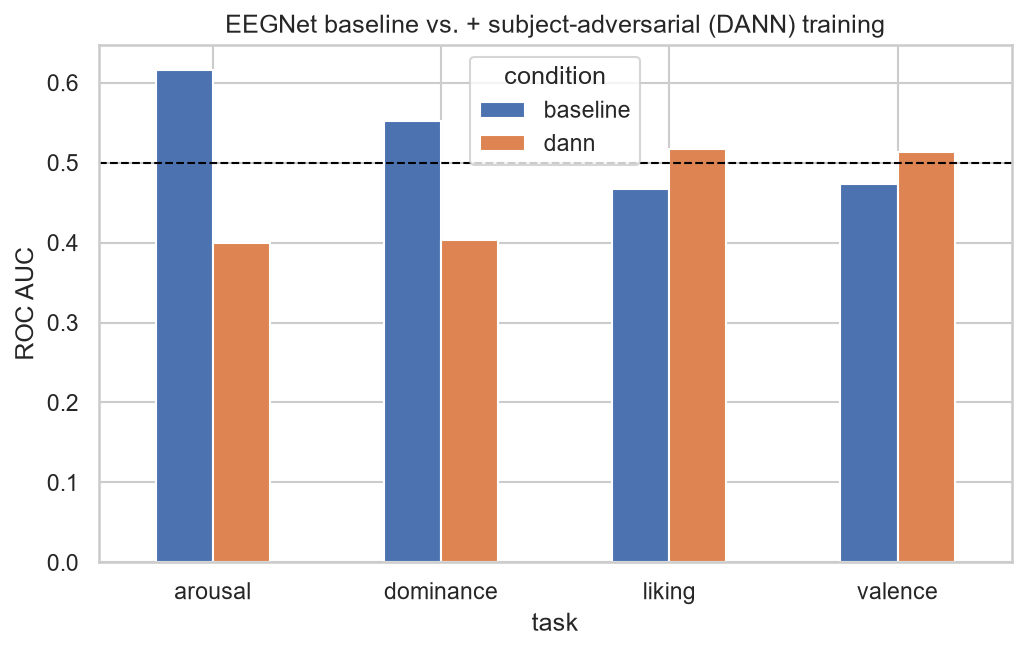
\includegraphics[width=0.85\textwidth]{track_b_domain_adversarial_auc.png}
\caption{DANN training --- ROC-AUC before/after, per task; note the
arousal/dominance collapse.}
\label{fig:dann}
\end{figure}

\section{Section 17 -- Five Deferred Literature Techniques}
\label{sec:s17}

\subsection{17.1 Euclidean Alignment}
\texttt{track\_a\_riemannian\_alignment.py} implements EA (He \& Wu 2019):
per subject, compute each window's raw spatial covariance
$C_i = X_i X_i^\top / T$, average across that subject's windows to get
$\bar R$, then whiten every window by $\bar R^{-1/2}$ \emph{before} DE
features are recomputed --- an upstream, per-subject, label-free,
raw-channel-level transform, unlike CORAL's downstream per-fold
feature-level operation. \textbf{Real result --- the strongest effect in the
whole project}: mean AUC delta $+0.044$ across 12 task/model combinations
(10/12 improved), and unlike every other alignment technique tried, the sign
is \emph{consistent} within three of the four tasks (valence +0.087/+0.027/+0.069,
arousal +0.078/+0.027/+0.065, dominance +0.074/+0.038/+0.073 across
LR/RF/XGBoost). Still modest in absolute terms (best post-EA AUCs land around
0.53--0.58).

\begin{table}[H]
\centering
\caption{Euclidean Alignment --- mean ROC-AUC across 3 models per task}
\label{tab:ea}
\begin{tabular}{lrrr}
\toprule
Task & No alignment & EA & $\Delta$ \\
\midrule
valence   & 0.467 & 0.528 & $+0.061$ \\
arousal   & 0.473 & 0.530 & $+0.057$ \\
dominance & 0.488 & 0.550 & $+0.062$ \\
liking    & 0.488 & 0.485 & $-0.003$ \\
\bottomrule
\end{tabular}
\end{table}

\begin{figure}[H]
\centering
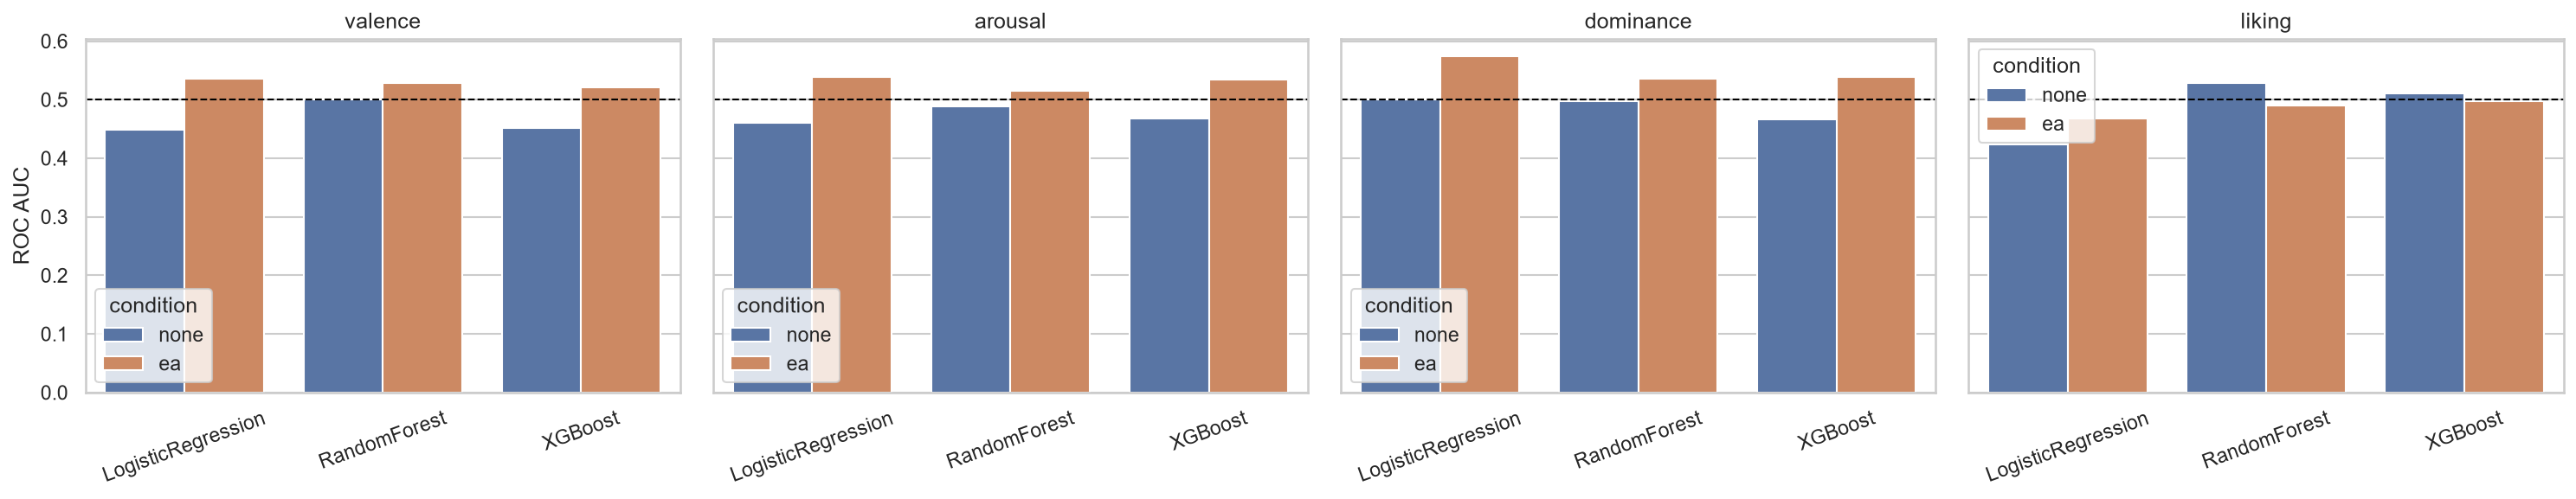
\includegraphics[width=0.85\textwidth]{track_a_riemannian_alignment_auc.png}
\caption{Euclidean Alignment --- ROC-AUC before/after, by model and task ---
the strongest effect found in the project.}
\label{fig:ea}
\end{figure}

\subsection{17.2 Self-supervised (TFR-style) pretraining}
\texttt{track\_b\_ssl\_pretrain.py} pretrains EEGNet's conv trunk with a
label-free MSE regression pretext task (predict each window's own
32-channel $\times$ 4-band log-band-power from the raw signal, training-fold
subjects only), then fine-tunes end-to-end, compared against an identically
trained scratch EEGNet. \textbf{Real result}: a bimodal, task-split pattern
--- valence AUC $0.474\to0.547$ ($+0.074$) and liking $0.467\to0.567$
($+0.100$) improved; arousal $0.616\to0.534$ ($-0.082$) and dominance
$0.552\to0.500$ ($-0.053$) got worse. The pretext task itself converged fine
(MSE dropped over 15 epochs), so this is not a training-failure artifact.

\begin{table}[H]
\centering
\caption{SSL pretraining --- ROC-AUC, EEGNet, single split}
\label{tab:ssl}
\begin{tabular}{lrrr}
\toprule
Task & Scratch & SSL-pretrained & $\Delta$ \\
\midrule
valence   & 0.474 & 0.547 & $+0.074$ \\
arousal   & 0.616 & 0.534 & $-0.082$ \\
dominance & 0.552 & 0.500 & $-0.053$ \\
liking    & 0.467 & 0.567 & $+0.100$ \\
\bottomrule
\end{tabular}
\end{table}

\begin{figure}[H]
\centering
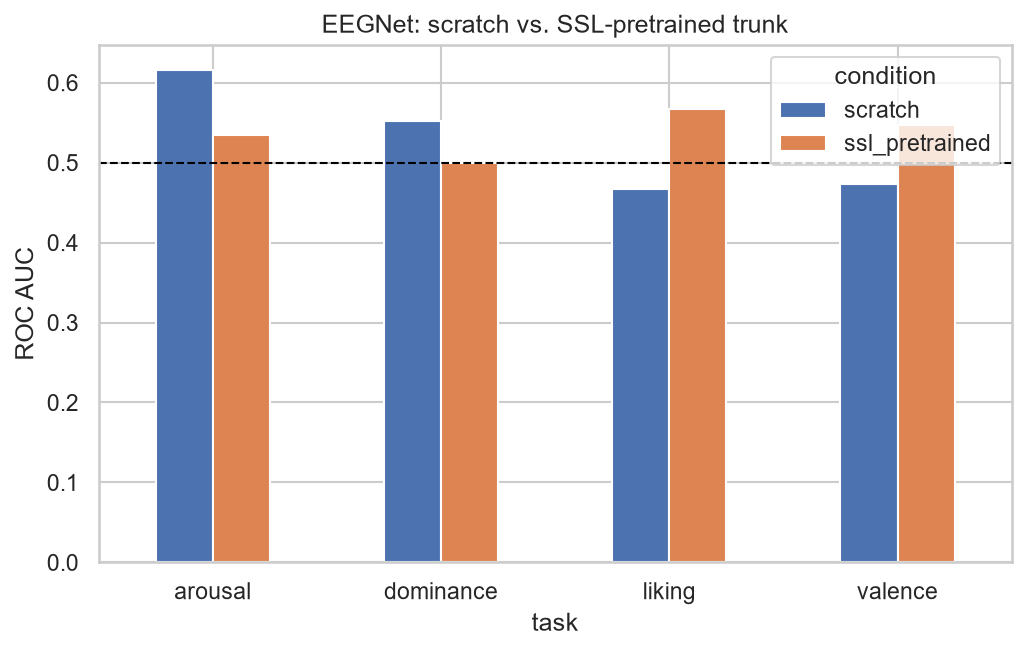
\includegraphics[width=0.85\textwidth]{track_b_ssl_pretrain_auc.png}
\caption{SSL pretraining --- ROC-AUC, scratch vs.\ pretrained, per task.}
\label{fig:ssl}
\end{figure}

\subsection{17.3 AUC-margin training loss}
\texttt{track\_b\_auc\_maximization.py} replaces cross-entropy with a
mini-batch pairwise squared-hinge AUC surrogate,
$L = \text{mean}_{i \in \text{pos}, j \in \text{neg}} \max(0, m - (s_i - s_j))^2$
(a simplified, self-contained version of the Ying et al.-style objective;
not the source paper's full saddle-point solver). \textbf{Real result}: the
one intervention with a clear, understood mechanism. Valence improved most
(AUC $0.474\to0.557$, $+0.083$) --- the cross-entropy baseline's 83.5\%
accuracy at 0.474 AUC was a textbook majority-class collapse; the AUC-margin
loss produced a far more balanced classifier (accuracy 0.507, AUC 0.557)
precisely because it is insensitive to that imbalance by construction.
Dominance improved slightly ($+0.008$); arousal ($-0.010$) and liking
($-0.018$) were small, likely-noise-level regressions.

\begin{table}[H]
\centering
\caption{AUC-margin loss --- ROC-AUC, EEGNet, single split}
\label{tab:aucmax}
\begin{tabular}{lrrr}
\toprule
Task & CE baseline & AUC-margin & $\Delta$ \\
\midrule
valence   & 0.474 & 0.557 & $+0.083$ \\
arousal   & 0.616 & 0.606 & $-0.010$ \\
dominance & 0.552 & 0.560 & $+0.008$ \\
liking    & 0.467 & 0.450 & $-0.018$ \\
\bottomrule
\end{tabular}
\end{table}

\begin{figure}[H]
\centering
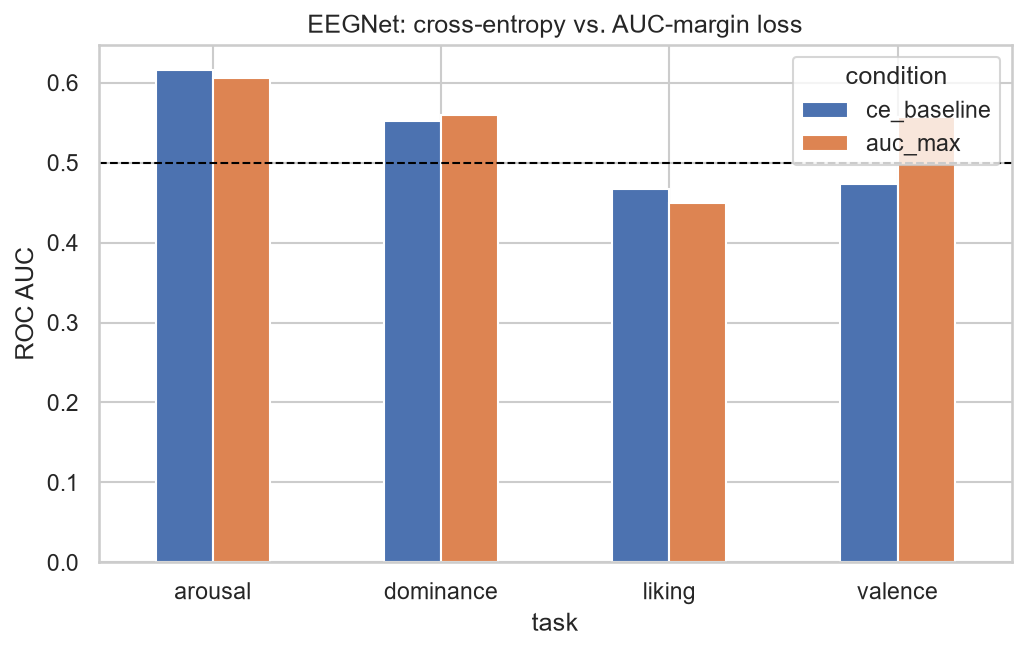
\includegraphics[width=0.85\textwidth]{track_b_auc_maximization_auc.png}
\caption{AUC-margin loss --- ROC-AUC, cross-entropy vs.\ AUC-margin, per
task.}
\label{fig:aucmax}
\end{figure}

\subsection{17.4 AdaBN test-time adaptation}
\texttt{track\_b\_test\_time\_adaptation.py} recomputes every BatchNorm
layer's running statistics using \emph{only} a held-out test subject's own
unlabelled windows (no gradients, no labels), then evaluates with the
adapted statistics. \textbf{Real result}: net negative overall. Arousal AUC
$0.616\to0.515$ ($-0.101$) and dominance $0.552\to0.489$ ($-0.063$) got
worse; liking $0.467\to0.549$ ($+0.082$) improved; valence was flat
($+0.002$). The only clearly net-negative intervention in Section 17.

\begin{table}[H]
\centering
\caption{AdaBN test-time adaptation --- ROC-AUC, EEGNet, single split}
\label{tab:adabn}
\begin{tabular}{lrrr}
\toprule
Task & No adaptation & AdaBN & $\Delta$ \\
\midrule
valence   & 0.474 & 0.476 & $+0.002$ \\
arousal   & 0.616 & 0.515 & $-0.101$ \\
dominance & 0.552 & 0.489 & $-0.063$ \\
liking    & 0.467 & 0.549 & $+0.082$ \\
\bottomrule
\end{tabular}
\end{table}

\begin{figure}[H]
\centering
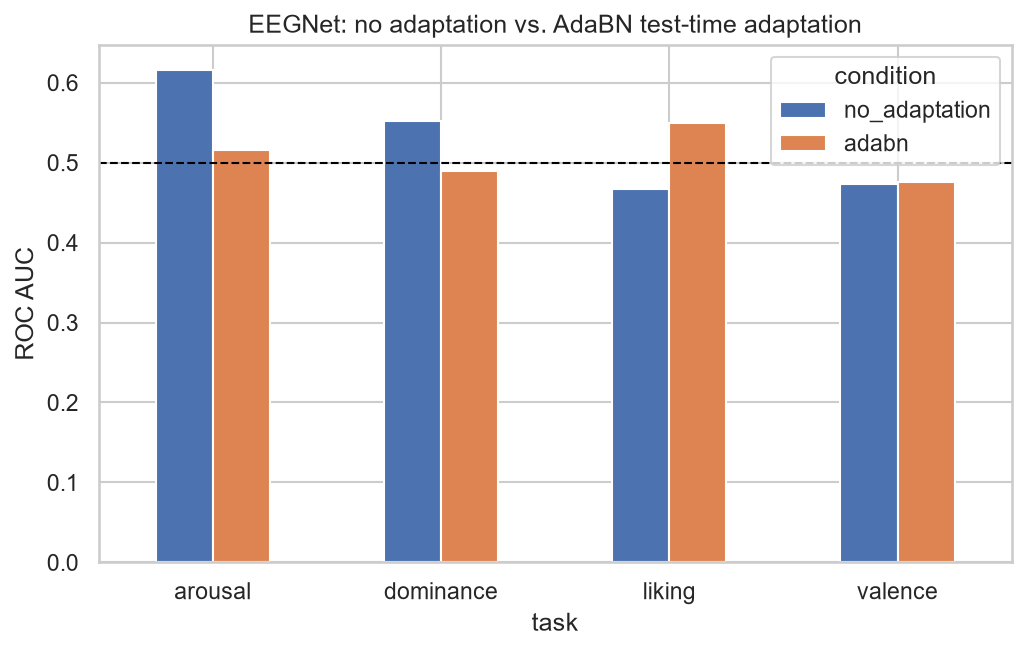
\includegraphics[width=0.85\textwidth]{track_b_test_time_adaptation_auc.png}
\caption{AdaBN test-time adaptation --- ROC-AUC before/after, per task.}
\label{fig:adabn}
\end{figure}

\subsection{17.5 SHAP interpretability diagnostic}
\texttt{track\_a\_shap\_diagnostic.py} fits XGBoost on the Full feature set
(one representative fold per task) and computes SHAP values on the held-out
fold via \texttt{shap.TreeExplainer}, aggregated by feature family and
individually. \textbf{Real result}: importance is spread across families
roughly in proportion to how many features each contributes, with two mild
departures --- DE's share (47--52\%) and Connectivity's (22--24\%) both sit
slightly above their feature-count share, while Hjorth's (21--26\%) sits
below. Notably, \textbf{frontal/hemispheric alpha asymmetry -- the one
feature family built around a named neurophysiological hypothesis -- carries
the smallest importance share in every task} (3.4--6.1\%). Top individual
features: \texttt{de\_beta\_P4} (valence), \texttt{de\_gamma\_FC2} (arousal
and liking), \texttt{plv\_beta\_F3-O1} (dominance) --- diffuse spectral/
connectivity structure, not FAA.

\begin{figure}[H]
\centering
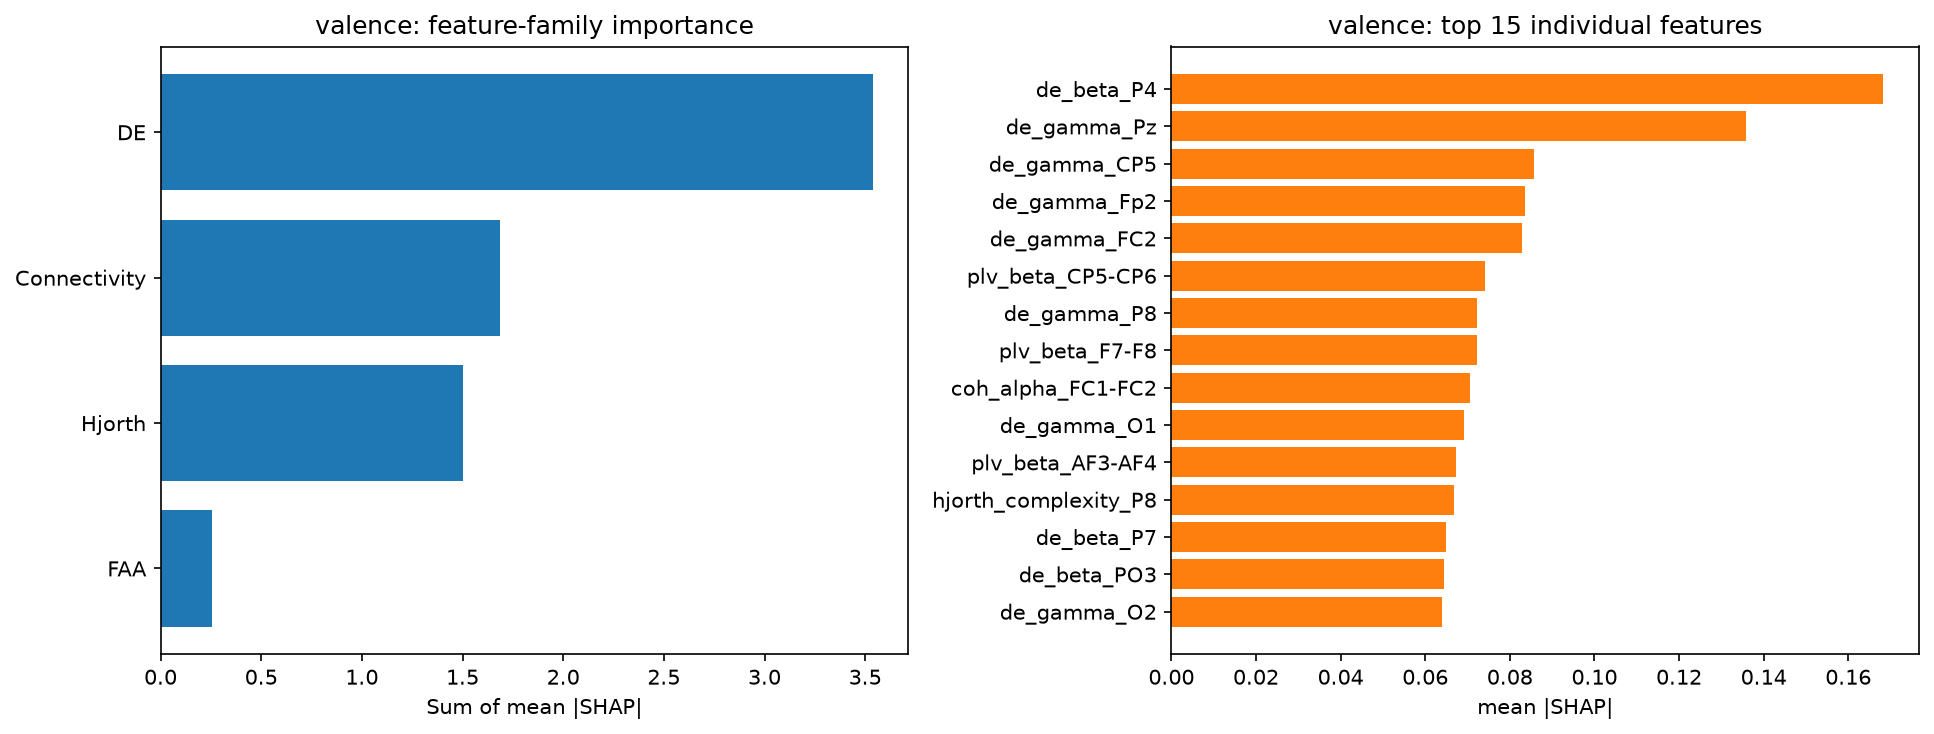
\includegraphics[width=0.8\textwidth]{track_a_shap_summary_valence.png}
\caption{SHAP summary --- valence (XGBoost, Full feature set, held-out fold).}
\label{fig:shap-valence}
\end{figure}

\begin{figure}[H]
\centering
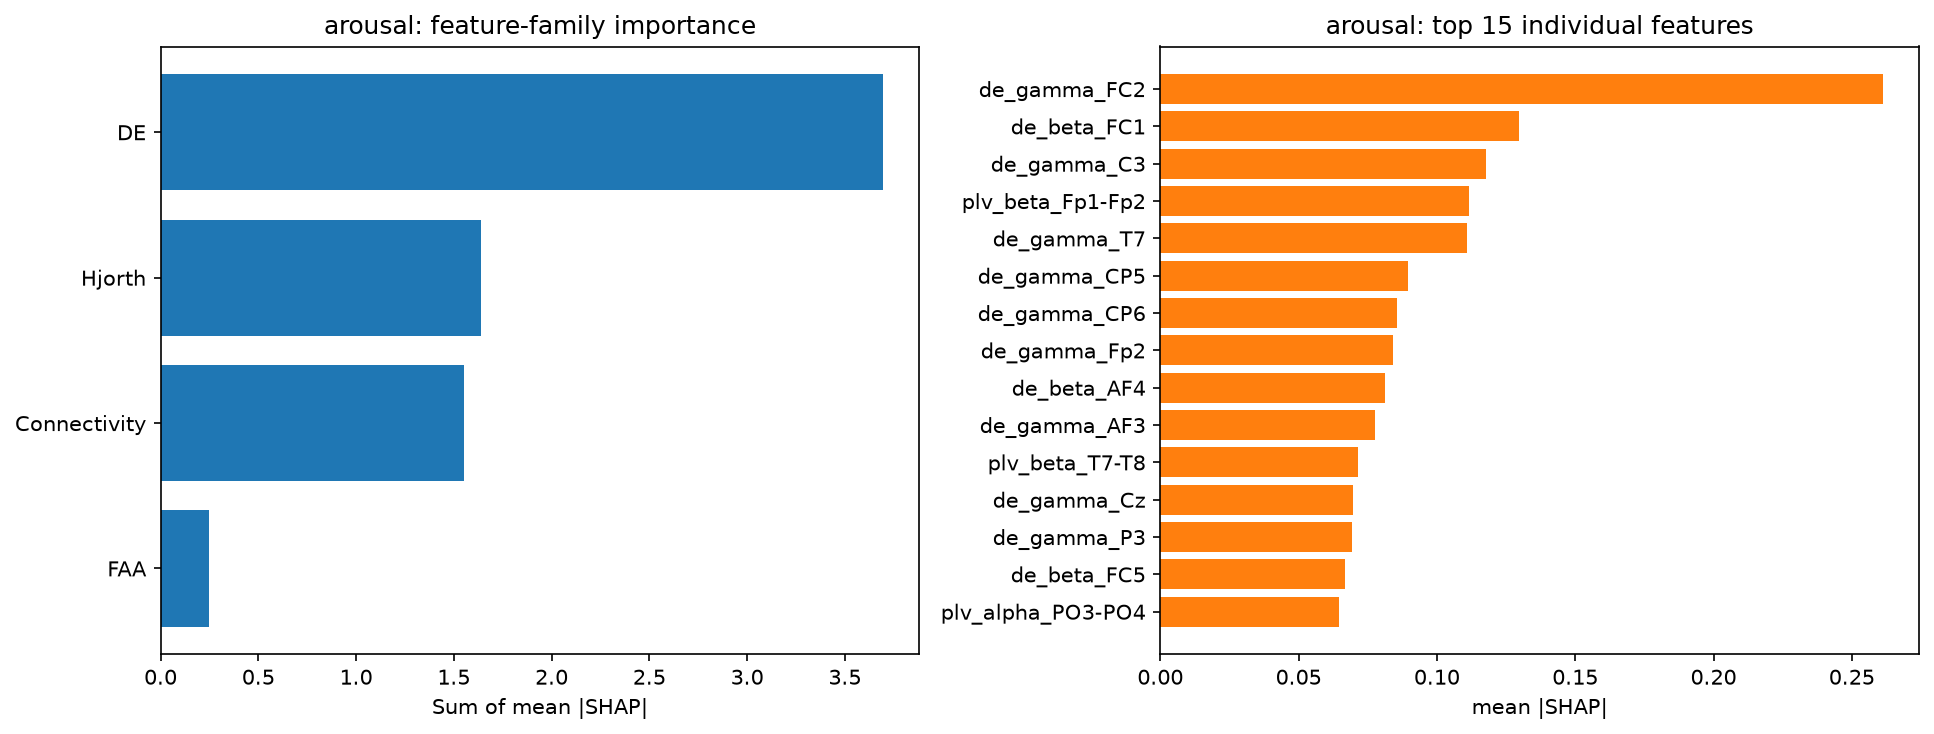
\includegraphics[width=0.8\textwidth]{track_a_shap_summary_arousal.png}
\caption{SHAP summary --- arousal.}
\label{fig:shap-arousal}
\end{figure}

\begin{figure}[H]
\centering
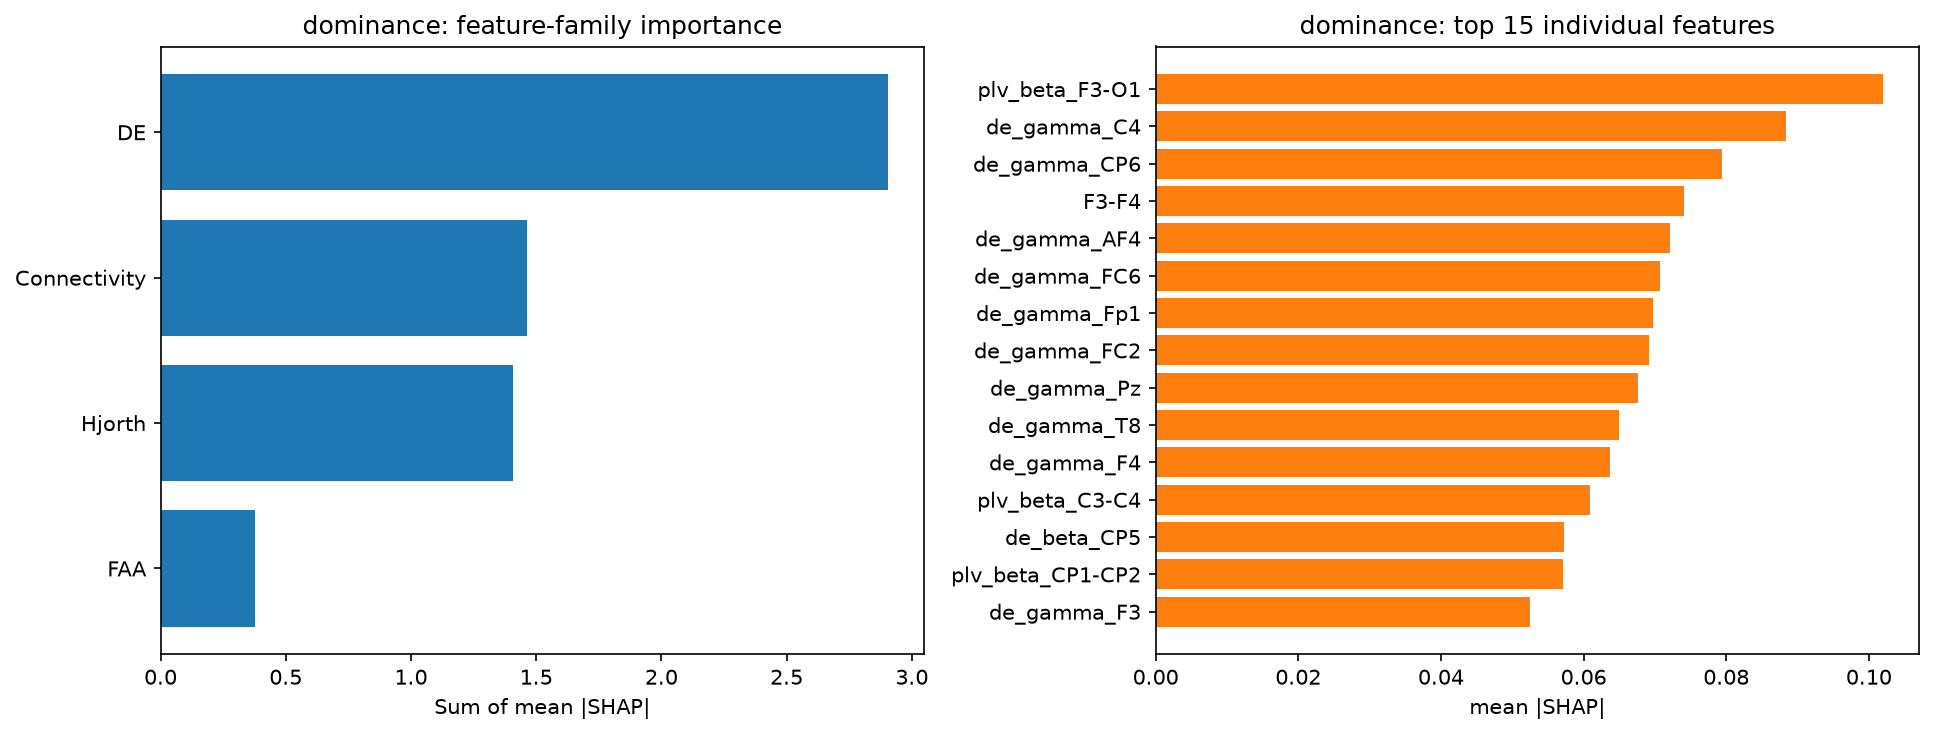
\includegraphics[width=0.8\textwidth]{track_a_shap_summary_dominance.png}
\caption{SHAP summary --- dominance.}
\label{fig:shap-dominance}
\end{figure}

\begin{figure}[H]
\centering
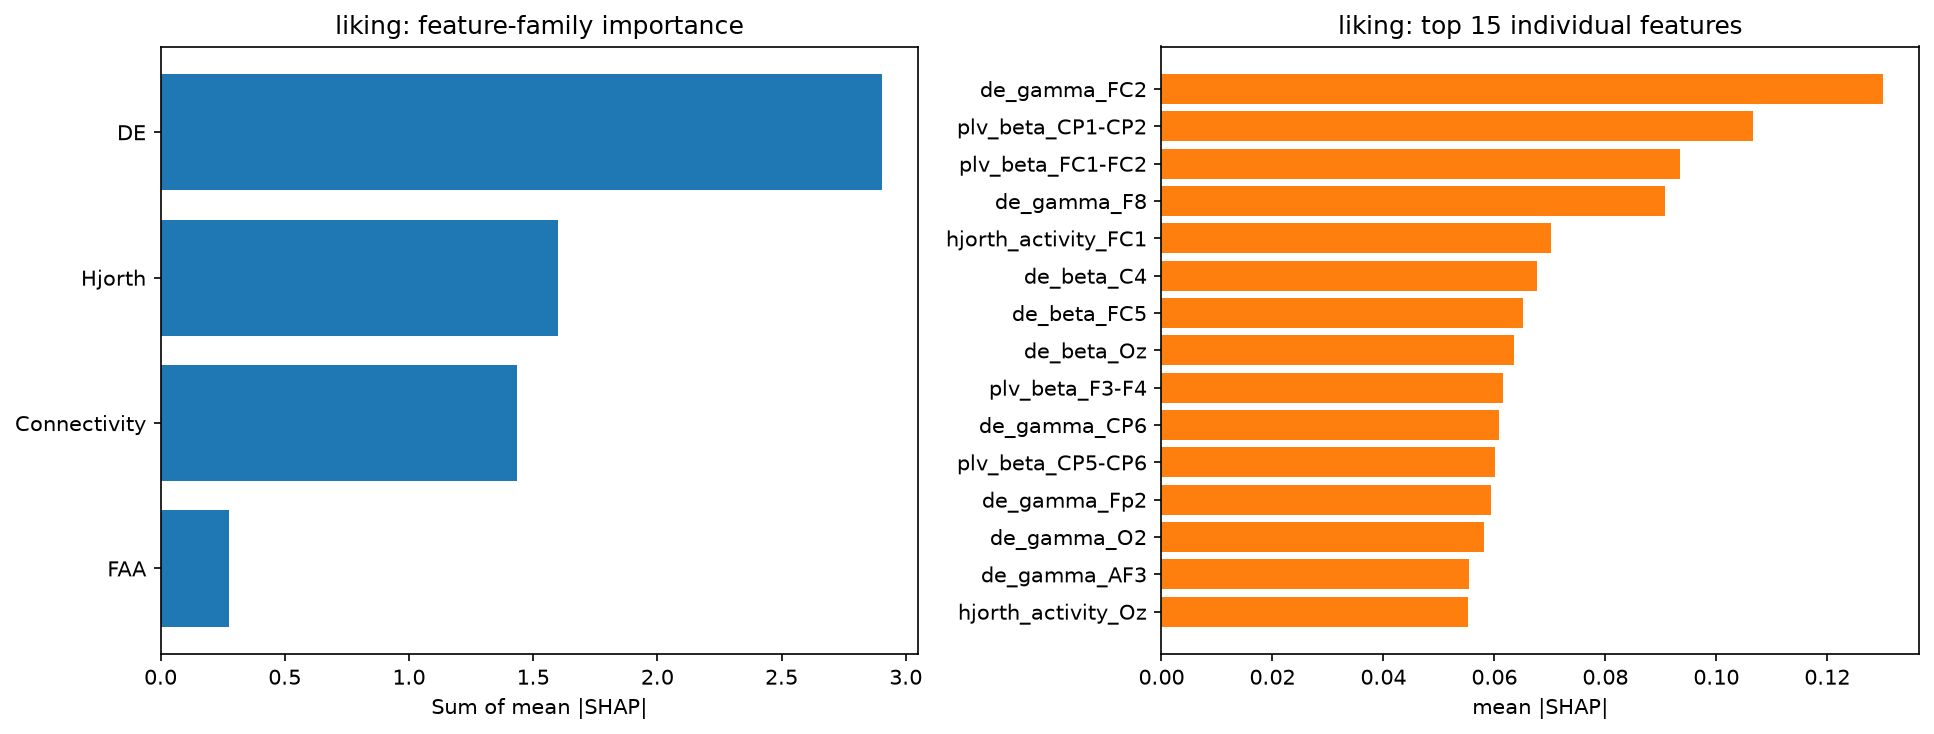
\includegraphics[width=0.8\textwidth]{track_a_shap_summary_liking.png}
\caption{SHAP summary --- liking.}
\label{fig:shap-liking}
\end{figure}

\section{Section 18 -- Does CORAL Stack on Top of Euclidean Alignment?}
\label{sec:s18}
\texttt{track\_a\_ea\_coral\_stacked.py} tests four conditions on the
DE-only feature set: \texttt{none}, \texttt{coral} alone, \texttt{ea} alone,
and \texttt{ea\_coral} (EA first, then CORAL on the resulting per-fold
split). \textbf{Real result --- it does not stack}. Mean AUC by condition:
EA alone 0.523, EA+CORAL 0.514, no-alignment baseline 0.479, CORAL alone
0.473 (CORAL alone is the \emph{worst} of the four on this feature set).
Adding CORAL on top of EA reduces AUC in 10/12 task/model combinations (mean
delta $-0.0093$). Interpretation: EA's per-subject raw-signal whitening
already removes most of the between-subject covariance structure CORAL is
also designed to correct, so CORAL's additional per-fold alignment acts on
residual structure that is mostly noise. \textbf{Practical takeaway: use EA
alone, not EA+CORAL.}

\begin{table}[H]
\centering
\caption{EA+CORAL stacking --- mean ROC-AUC by condition, DE-only feature
set, across 4 tasks $\times$ 3 models (12 fits)}
\label{tab:ea-coral-stacked}
\begin{tabular}{lr}
\toprule
Condition & Mean ROC-AUC \\
\midrule
none (no alignment) & 0.479 \\
CORAL alone          & 0.473 \\
EA alone             & 0.523 \\
EA + CORAL           & 0.514 \\
\bottomrule
\end{tabular}
\end{table}

\begin{figure}[H]
\centering
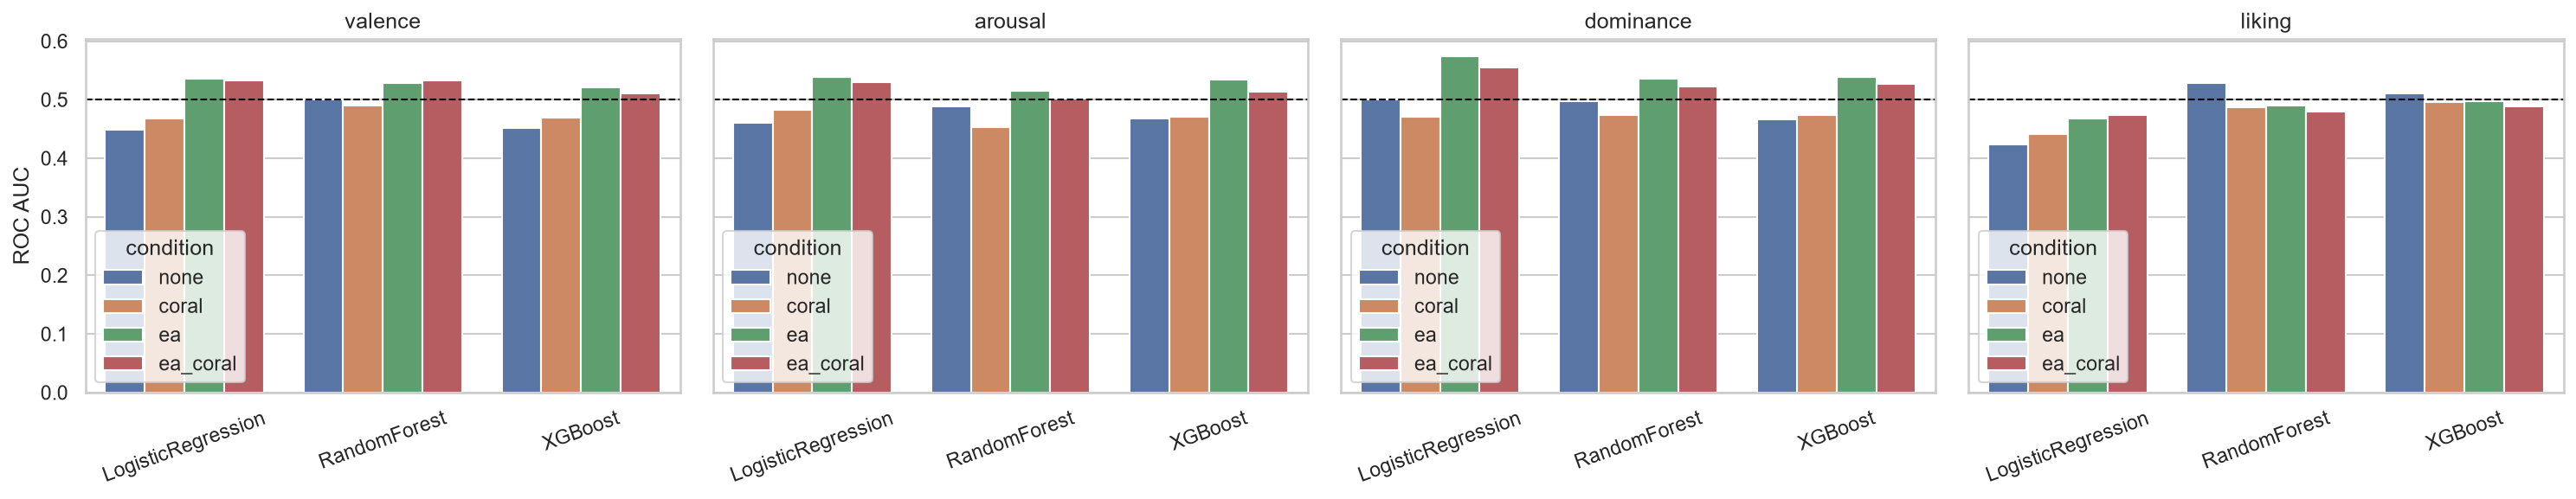
\includegraphics[width=0.85\textwidth]{track_a_ea_coral_stacked_auc.png}
\caption{EA+CORAL stacking --- ROC-AUC by condition, model, and task.}
\label{fig:ea-coral-stacked}
\end{figure}

\section{Addendum: EEG Overview QC Section (added post-hoc)}
\label{sec:eeg-overview}
A small-multiples quality-control plot was added between Sections 2 and 3
during this project: an $8\times4$ grid, one panel per subject, each showing
all 32 channels of that subject's baseline-normalised trial-1 EEG stacked
with a fixed vertical offset, in a single neutral ink colour (per-channel
colour-coding was deliberately avoided --- with 32 overlapping traces per
panel, colour cannot carry per-channel identity meaningfully, and would
violate the categorical-colour design principle of assigning one hue per
identifiable series). This is a visual sanity check, not an analysis: it
lets a reader spot subjects with obviously flat, saturated, or anomalously
noisy channels before trusting downstream numbers for them.

\begin{figure}[H]
\centering
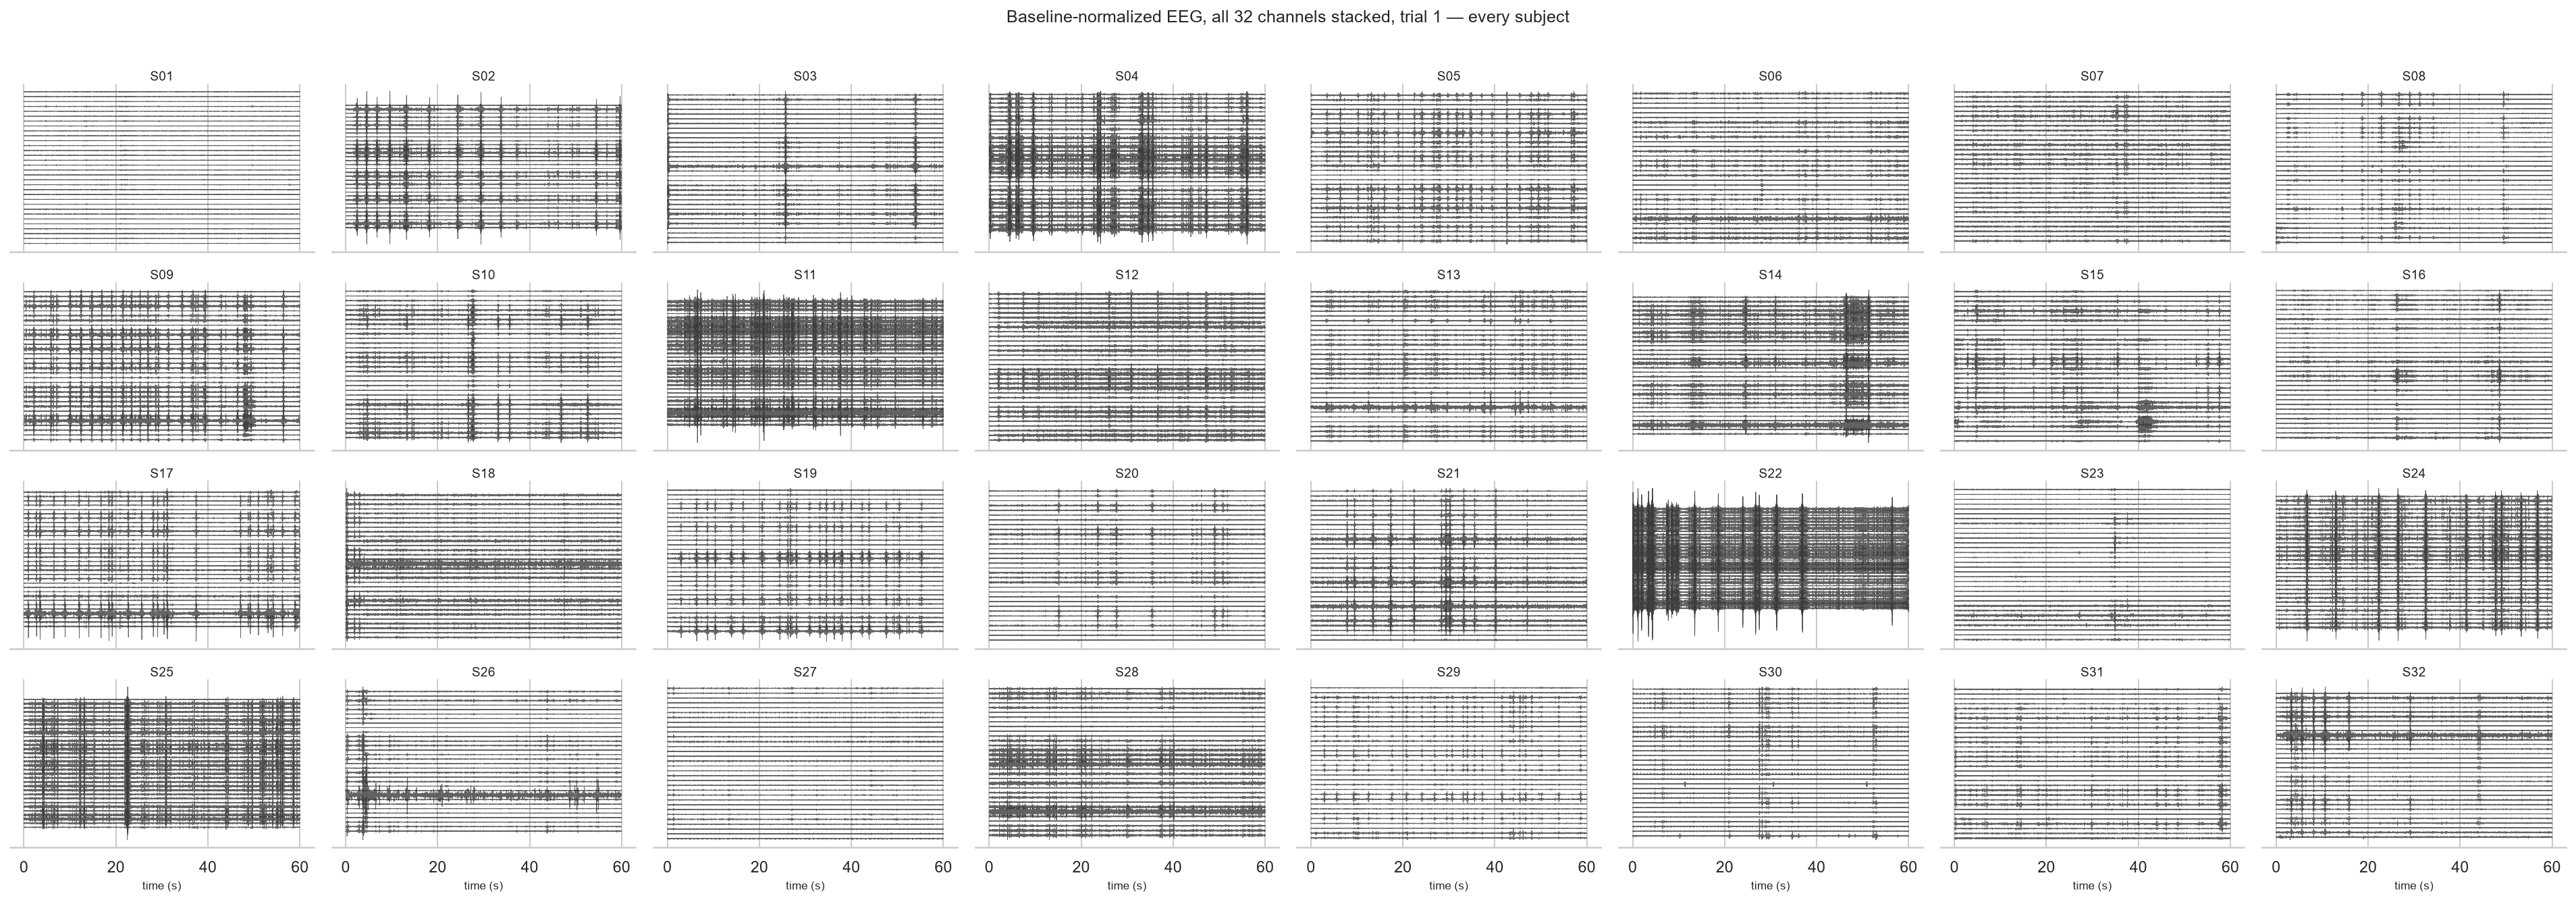
\includegraphics[width=\textwidth]{eeg_overview_all_subjects.png}
\caption{EEG overview QC grid --- baseline-normalised trial-1 EEG, all 32
channels, one panel per subject (8$\times$4 grid).}
\label{fig:eeg-overview}
\end{figure}

\chapter{Companion Scripts Reference}
\label{ch:scripts}

Every experiment in Sections~\ref{sec:s9}--\ref{sec:s18} that was too
expensive to run inline in the notebook lives in its own standalone script
under \texttt{scripts/}, each writing one CSV to \texttt{results/tables/}
(and, where relevant, PNGs to \texttt{results/figures/}) that the notebook
then reads and displays. This chapter documents each script's function.

\section{Feature/dataset builders}
\begin{description}
  \item[\texttt{dl\_models.py}] Canonical PyTorch definitions of EEGNet,
        ShallowConvNet, CNN-LSTM, and TSception, plus the hemisphere-pair
        channel indices TSception needs. Imported by every
        \texttt{track\_b\_*.py} script so the architectures are defined
        exactly once, not re-implemented per script.
  \item[\texttt{rich\_features.py}] Implements Hjorth parameters
        (\texttt{compute\_hjorth}), frontal/hemispheric alpha asymmetry
        (\texttt{compute\_alpha\_asymmetry}), and PLV/coherence connectivity
        (\texttt{compute\_connectivity}, via a from-scratch Hilbert-transform
        phase-locking-value computation and a Welch-style
        magnitude-squared-coherence estimator). Includes a
        \texttt{if\_\_name\_\_=="\_\_main\_\_"} self-test against synthetic
        data (shape checks, $[0,1]$-boundedness for PLV/coherence, and an
        index-math cross-check for FAA) that must pass before the module is
        trusted for the real build.
  \item[\texttt{build\_extended\_features.py}] Runs \texttt{rich\_features.py}
        (plus DE) over all 32 DEAP subjects, producing
        \texttt{deap\_features\_ext\_v1.npz} (295-dim Full feature set,
        19{,}200 windows). Its DE computation is verified to match the
        original cache byte-for-byte before the richer features are trusted.
  \item[\texttt{build\_overlap\_windows.py}] Rebuilds the raw-window Track B
        dataset with 50\% stride overlap
        (\texttt{deap\_windows\_4s\_overlap50\_32subj\_v1.npz}, 37{,}120
        windows), for Section~\ref{sec:s11}.
  \item[\texttt{build\_raw\_ratings.py}] Extracts the raw continuous 1--9
        SAM ratings per window, row-aligned 1:1 with the extended feature
        cache (verified via an explicit \texttt{groups} array equality
        assertion), for Section~\ref{sec:s14}'s label-cleanup variants.
\end{description}

\section{Track A companion scripts}
\begin{description}
  \item[\texttt{track\_a\_ablation.py}] Section~\ref{sec:s9}: 6 feature-set
        combinations $\times$ 3 models $\times$ 4 tasks, \texttt{GroupKFold(5)}.
  \item[\texttt{track\_a\_repeated\_nested\_cv.py}] Section~\ref{sec:s10}:
        5$\times$-repeated \texttt{GroupKFold} for all 6 models (with a
        custom subject-relabeling generator, \texttt{repeated\_group\_}\linebreak
        \texttt{kfold\_splits}, since \texttt{sklearn} has no
        \texttt{RepeatedGroupKFold}) plus nested
        \texttt{GroupKFold(3)}/\texttt{RandomizedSearchCV} hyperparameter
        search for XGBoost and RandomForest.
  \item[\texttt{track\_a\_label\_cleanup.py}] Section~\ref{sec:s14}: the
        three label-binarisation variants (\texttt{raw\_threshold},
        \texttt{per\_subject\_z}, \texttt{drop\_middle}).
  \item[\texttt{track\_a\_calibration\_loso.py}] Section~\ref{sec:s15}: true
        32-fold LOSO with an 80/20 per-subject eval/calibration trial split
        and XGBoost warm-start (\texttt{xgb\_model=} continuation boosting).
  \item[\texttt{track\_a\_significance\_test.py}] Section~\ref{sec:s16}.1:
        300-permutation label-shuffle null-distribution test, parallelised
        across CPU cores with \texttt{joblib.Parallel}.
  \item[\texttt{track\_a\_domain\_alignment.py}] Section~\ref{sec:s16}.2:
        CORAL alignment (\texttt{coral\_align}, via
        \texttt{\_sym\_matrix\_power} eigendecomposition).
  \item[\texttt{track\_a\_riemannian\_alignment.py}] Section~\ref{sec:s17}.1:
        Euclidean Alignment (\texttt{euclidean\_align}), operating on raw
        windows before DE recomputation.
  \item[\texttt{track\_a\_shap\_diagnostic.py}] Section~\ref{sec:s17}.5:
        \texttt{shap.TreeExplainer} on one representative fold per task,
        aggregated by feature and by family, with bar-chart figures saved
        per task.
  \item[\texttt{track\_a\_ea\_coral\_stacked.py}] Section~\ref{sec:s18}: the
        4-condition (\texttt{none}/\texttt{coral}/\texttt{ea}/\texttt{ea\_coral})
        stacking test, re-implementing both \texttt{euclidean\_align} and
        \texttt{coral\_align} locally so this script is self-contained.
\end{description}

\section{Track B companion scripts}
\begin{description}
  \item[\texttt{track\_b\_repeated.py}] Section~\ref{sec:s11}: 5-seed
        repeated subject-independent splits, both window variants, all 4
        architectures $\times$ 4 tasks (160 runs).
  \item[\texttt{track\_b\_domain\_adversarial.py}] Section~\ref{sec:s16}.3:
        \texttt{GradReverse} autograd function, \texttt{EEGNetDANN} (reuses
        EEGNet's conv blocks, adds a GRL + domain-classifier branch), and
        the Ganin \& Lempitsky progressive-$\lambda$ training loop.
  \item[\texttt{track\_b\_ssl\_pretrain.py}] Section~\ref{sec:s17}.2:
        \texttt{EEGNetSSL} (shares EEGNet's trunk, regression head for the
        DE-prediction pretext task), a 15-epoch label-free pretraining
        stage, then fine-tuning; the training/val/test split is computed
        once and reused across all four tasks (compute optimisation, not a
        methodological shortcut, since the split depends only on
        \texttt{groups}/\texttt{seed}, not on labels).
  \item[\texttt{track\_b\_auc\_maximization.py}] Section~\ref{sec:s17}.3:
        \texttt{auc\_margin\_loss}, a drop-in loss-function swap with
        everything else (model, split, seed) held identical to the
        cross-entropy baseline.
  \item[\texttt{track\_b\_test\_time\_adaptation.py}] Section~\ref{sec:s17}.4:
        \texttt{reset\_bn\_for\_adaptation} (zeroes BatchNorm running stats,
        sets momentum to \texttt{None} for a true cumulative average) and
        \texttt{adabn\_predict\_one\_subject} (2 label-free adaptation
        epochs per test subject, under \texttt{torch.no\_grad()}).
\end{description}

\section{Cross-corpus scripts}
See Section~\ref{sec:seed-iv-adapter} for \texttt{base.py},
\texttt{seed\_adapter.py}, and \texttt{run\_cross\_corpus.py}.

\section{Notebook-authoring scripts}
\texttt{update\_notebook.py} through \texttt{update\_notebook\_v5.py} are
historical, versioned scripts used to programmatically author/update the
notebook's markdown and code cells during earlier stages of the project
(each is a one-off generator, not re-run as part of the analysis pipeline
itself). They are kept as a record of how the notebook's content evolved
but are not part of the reproducible-results path.

\chapter{Literature Review and Paper Attribution}
\label{ch:literature}

\section{Corpus}
\texttt{D:\textbackslash EEG\textbackslash papers\_EEG\textbackslash} contains 32 PDFs, renamed
during this project from their original arXiv-ID/journal-slug filenames to
their full paper titles for readability. Table~\ref{tab:papers-cited} lists
the papers with an \textbf{explicit, documented} role in this project's code
or notebook text --- i.e.\ named in a script's docstring or a notebook
markdown cell as the specific motivation for a specific experiment.

\begin{longtable}{p{4.7cm}p{4.3cm}p{5.5cm}}
\caption{Papers with an explicit, documented contribution to this project}
\label{tab:papers-cited} \\
\toprule
Paper (short ref.) & Used in & Why \\
\midrule
\endfirsthead
\toprule
Paper (short ref.) & Used in & Why \\
\midrule
\endhead
The Role of Review Process Failures in Affective State Estimation: An
Empirical Investigation of DEAP Dataset (Khan et al.) &
Sec.\ 16.1, \texttt{track\_a\_significance\_test.py} &
Documents that DEAP pipelines can look deceptively strong under leaky
evaluation even on a label-randomised (``watermelon'') control; motivated
building a genuine permutation-null significance test for this project's
own already-correct \texttt{GroupKFold} protocol. \\
\addlinespace
Domain Adaptation and Generalization on Functional Medical Images: A
Systematic Survey &
Sec.\ 16.2 \& 17.1, \texttt{track\_a\_domain\_alignment.py},
\texttt{track\_a\_riemannian\_alignment.py}, \texttt{track\_b\_domain\_}\linebreak
\texttt{adversarial.py} &
Surveys CORAL and Euclidean Alignment as standard, cheap, unsupervised
domain-adaptation remedies for distribution shift; also one of six sources
converging on adversarial subject-invariance (DANN). \\
\addlinespace
DS-AGC: Semi-Supervised Dual-Stream Self-Attentive Adversarial Graph
Contrastive Learning for Cross-Subject EEG Emotion Recognition &
Sec.\ 16.2 \& 17.1, same scripts as above &
Reports plain CORAL reaching $\sim$65--70\% under LOSO on SEED where
untransformed features stay under 60\% --- the concrete empirical precedent
that motivated testing CORAL and EA here (though this project's own CORAL
result did not replicate that scale of gain). \\
\addlinespace
PARSE: Pairwise Alignment of Representations in Semi-Supervised EEG Learning
for Emotion Recognition &
Sec.\ 16.3, \texttt{track\_b\_domain\_adversarial.py} &
One of six independently-converging sources recommending a gradient-
reversal-layer domain discriminator for subject-invariant EEG
representation learning. \\
\addlinespace
EEG Based Emotion Recognition: A Tutorial and Review &
Sec.\ 16.3, \texttt{track\_b\_domain\_adversarial.py} &
Same DANN motivation as above. \\
\addlinespace
Graph Neural Networks in EEG-Based Emotion Recognition: A Survey &
Sec.\ 16.3, \texttt{track\_b\_domain\_adversarial.py} &
Same DANN motivation as above (the ``GNN survey'' source). \\
\addlinespace
Deep Learning-Based EEG Emotion Recognition: A Review (\texttt{brainsci-16-00041}) &
Sec.\ 16.3, \texttt{track\_b\_domain\_adversarial.py} &
Same DANN motivation as above. \\
\addlinespace
A Review of Deep Learning Techniques for EEG-Based Emotion Recognition:
Models, Methods, and Datasets (PRISMA review, \texttt{f1000research-14-196597}) &
Sec.\ 16.3 result discussion &
Names ``over-aggressive alignment collapsing class structure'' as a
documented UDA failure pattern --- matched exactly by this project's own
DANN arousal/dominance collapse, used to interpret (not just report) that
result. \\
\addlinespace
Cascaded Self-Supervised Learning for Subject-Independent EEG-Based
Emotion Recognition &
Sec.\ 17.2, \texttt{track\_b\_ssl\_pretrain.py} &
The single paper in the whole review evaluated LOSO on DEAP itself while
beating domain-adaptation baselines --- the strongest outside evidence that
a pretraining stage (not a training-time loss/architecture change) could
move this project's subject-independent AUC. \\
\addlinespace
Self-Supervised Learning for Electroencephalogram: A Systematic Survey &
Sec.\ 17.2, \texttt{track\_b\_ssl\_pretrain.py} &
Corroborating survey context for the SSL-pretraining design. \\
\addlinespace
Electroencephalogram Emotion Recognition via AUC Maximization (Xiao) &
Sec.\ 17.3, \texttt{track\_b\_auc\_maximization.py} &
The most directly on-metric deferred idea: this project's own headline
metric is ROC-AUC, so a loss that directly targets AUC (rather than
per-sample cross-entropy) is a natural, cheap intervention to test. \\
\addlinespace
Towards Practical Emotion Recognition: An Unsupervised Source-Free Approach
for EEG Domain Adaptation &
Sec.\ 17.4, \texttt{track\_b\_test\_time\_adaptation.py} &
Surveys the source-free UDA family (of which AdaBN is the cheapest,
most-established member) as the natural target-aware follow-up to DANN. \\
\addlinespace
Enhancing EEG-Based Emotion Detection with Hybrid Models: Insights from
DEAP Dataset Applications (\texttt{sensors-25-01827}) &
Sec.\ 17.5, \texttt{track\_a\_shap\_diagnostic.py} &
Logged the SHAP interpretability diagnostic as a cheap, never-run check on
whether near-chance models lean on plausible or noise-like features. \\
\bottomrule
\end{longtable}

\section{Papers in the corpus without a documented individual attribution}
\label{sec:literature-gap}
The remaining 19 papers in \texttt{papers\_EEG/} were assembled as part of
the ``31 papers spanning EEG-emotion surveys, domain-adaptation/
generalization methods, contrastive/self-supervised pretraining,
GAN/diffusion augmentation, and DEAP-specific methodology critiques'' that
Section~16's markdown describes as having been ``read end-to-end by
parallel literature-extraction passes.'' \textbf{Every script above and the
notebook's own Section 16/17 text repeatedly refer to a file,
\texttt{D:\textbackslash EEG\textbackslash papers\_EEG\textbackslash literature\_log.txt}, described
as containing ``full attribution --- what was taken from each paper, why it
was or wasn't used, and how it maps to the scripts above.'' This file did
not exist anywhere in the project directory at the time this report was
first drafted, despite being referenced by name at least eight times across
the notebook and scripts.}

\textbf{Update: this gap has since been closed.} The log was reconstructed
by opening all 32 PDFs directly (title, abstract, and opening paragraphs)
and is now saved at \texttt{D:\textbackslash EEG\textbackslash literature\_log.txt} (note: at
the project root, not inside \texttt{papers\_EEG/} where the original
in-code references point --- update those references or move the file if
strict path consistency with the existing docstrings is wanted). It
confirms the 13 papers in Table~\ref{tab:papers-cited} above as the only
ones with a genuine code-level attribution, and gives each of the remaining
19 an abstract-grounded one-paragraph summary plus an honest
``reviewed, not implemented'' status with a stated reason, so their
inclusion in the corpus is now explainable even though none of them
produced code:
\begin{itemize}[itemsep=0pt]
  \item Spatial-Temporal Transformers for EEG Emotion Recognition
  \item A Two-Stage Efficient 3-D CNN Framework for EEG Based Emotion Recognition
  \item Towards Emotion Recognition for Virtual Environments: An Evaluation
        of EEG Features on Benchmark Dataset
  \item AMDET: Attention Based Multiple Dimensions EEG Transformer for
        Emotion Recognition
  \item Emotion Recognition Based on Multi-Modal Electrophysiology
        Multi-Head Attention Contrastive Learning
  \item Self-Supervised Group Meiosis Contrastive Learning for EEG-Based
        Emotion Recognition
  \item Enhancing EEG Signal-Based Emotion Recognition with Synthetic Data:
        Diffusion Model Approach
  \item A Comprehensive Survey on EEG-Based Emotion Recognition: A
        Graph-Based Perspective
  \item EEG-SCMM: Soft Contrastive Masked Modeling for Cross-Corpus
        EEG-Based Emotion Recognition
  \item A Novel Fourier Adjacency Transformer for Advanced EEG Emotion
        Recognition
  \item LEL: Lipschitz Continuity Constrained Ensemble Learning for
        Efficient EEG-Based Intra-Subject Emotion Recognition
  \item EEG Emotion Recognition Through Deep Learning
  \item Three-Way Emotion Classification of EEG-Based Signals Using Machine
        Learning
  \item EEG Feature Extraction and Data Augmentation in Emotion Recognition
  \item Emotion Recognition Based on EEG Using Generative Adversarial Nets
        and Convolutional Neural Network
  \item ERTNet: An Interpretable Transformer-Based Framework for EEG
        Emotion Recognition
  \item EEG-Based Emotion Recognition Systems: Comprehensive Study (\texttt{main.pdf})
  \item Detecting Emotions Through EEG Signals Based on Modified
        Convolutional Fuzzy Neural Network
  \item EEG-Based Smart Emotion Recognition Using Meta-Heuristic
        Optimization and Hybrid Deep Learning Techniques
\end{itemize}
Note: ``Enhancing EEG-Based Emotion Detection with Hybrid Models: Insights
from DEAP Dataset Applications'' is the one explicitly-cited paper from this
topical area (Section~17.5, Table~\ref{tab:papers-cited}); some titles above
overlap topically with cited papers without being the cited instance
themselves.

\textbf{Recommendation}: with the log now reconstructed, decide whether to
keep the full 32-paper corpus (citing the 19 reviewed-but-unused papers as
general background/related work, correctly labelled as such) or trim
\texttt{papers\_EEG/} down to the 13 papers that actually drove an
implemented experiment, to keep a future bibliography tight. See
\texttt{literature\_log.txt} for the full per-paper summaries and reasoning
behind each status.

\chapter{Consolidated Results}
\label{ch:results}

Table~\ref{tab:master} consolidates the headline AUC numbers across every
experiment in the notebook, in chronological/section order. All numbers are
mean ROC-AUC unless noted; ``$\Delta$'' is the change versus that
experiment's own stated control condition.

\begin{longtable}{p{5.5cm}p{2.3cm}p{2.1cm}p{4.3cm}}
\caption{Master results table} \label{tab:master} \\
\toprule
Experiment (section) & Best/observed AUC & $\Delta$ vs.\ control & Verdict \\
\midrule
\endfirsthead
\toprule
Experiment (section) & Best/observed AUC & $\Delta$ vs.\ control & Verdict \\
\midrule
\endhead
Track A best model (\S5) & 0.501--0.534 & --- & near chance \\
Track B best model (\S6) & 0.475--0.607 & --- & near chance, mixed by task \\
Feature-set ablation (\S9) & 0.478--0.494 (means) & $\le0.016$ across sets & no feature set helps \\
Repeated GroupKFold (\S10) & 15/24 CIs contain 0.5 & --- & mostly chance-consistent \\
Nested CV (\S10) & 0.454--0.524 & $\approx0$ vs.\ fixed HP & tuning is not the bottleneck \\
Window overlap (\S11) & 0.483 vs.\ 0.498 & $+0.015$ & inconsistent, not real gain \\
Cross-corpus DEAP baseline (\S12) & 0.452 & --- & weakest of the three settings \\
Cross-corpus zero-shot (\S12) & 0.517 & $+0.065$ vs.\ DEAP baseline & modest, above chance \\
Cross-corpus SEED-IV LOSO (\S12) & \textbf{0.673} & $+0.221$ vs.\ DEAP baseline & \textbf{real, moderate signal} \\
Label cleanup, per\_subject\_z (\S14) & 0.514 (mean) & $+0.031$ vs.\ raw & modest, confounded by rebalancing \\
Calibration, arousal (\S15) & 0.577 & $+0.071$ vs.\ zero-shot & real, modest personalisation effect \\
Permutation test, dominance (\S16.1) & 0.561 & $z=+12.3$, $p=0.0033$ & significant but small \\
Permutation test, others (\S16.1) & 0.437--0.458 & $p=1.0$ (all 3) & indistinguishable from chance \\
CORAL (\S16.2) & mean $\Delta+0.0059$ & 8/12 up, 4/12 down & no stable effect \\
DANN, valence/liking (\S16.3) & $+0.039$/$+0.050$ & --- & small gains \\
DANN, arousal/dominance (\S16.3) & $-0.216$/$-0.149$ & --- & \textbf{collapse} \\
Euclidean Alignment (\S17.1) & mean $\Delta+0.044$ & 10/12 up & \textbf{strongest effect overall} \\
SSL pretraining (\S17.2) & $+0.074$/$+0.100$ (val/lik) & $-0.082$/$-0.053$ (aro/dom) & bimodal task split \\
AUC-margin loss (\S17.3) & $+0.083$ (valence) & mixed elsewhere & mechanistically understood win \\
AdaBN (\S17.4) & $+0.082$ (liking) & $-0.101$/$-0.063$ (aro/dom) & net negative \\
SHAP diagnostic (\S17.5) & --- & --- & diffuse importance, FAA weakest \\
EA+CORAL stacking (\S18) & EA 0.523 vs.\ EA+CORAL 0.514 & $-0.0093$ & \textbf{does not stack; use EA alone} \\
\bottomrule
\end{longtable}

\section{Figures}
All 24 figures in \texttt{results/figures/} are embedded in place in
Chapter~\ref{ch:notebook}, alongside the section that produced them (see
List of Figures, p.~\pageref{fig:class-balance}, for the full index). The
most important for a final report remain \texttt{class\_balance.png}
(Fig.~\ref{fig:class-balance}, \S4),
\texttt{track\_a\_accuracy.png}/\texttt{combined\_accuracy\_comparison.png}
(Figs.~\ref{fig:track-a-accuracy}/\ref{fig:combined-accuracy}, \S5--7),
\texttt{track\_a\_repeated\_cv\_auc\_ci.png} (Fig.~\ref{fig:repeated-cv},
\S10), \texttt{track\_a\_riemannian\_alignment\_auc.png}
(Fig.~\ref{fig:ea}, \S17.1, the strongest result),
\texttt{track\_a\_ea\_coral\_stacked\_auc.png}
(Fig.~\ref{fig:ea-coral-stacked}, \S18), and
\texttt{cross\_corpus\_deap\_seediv.png} (Fig.~\ref{fig:cross-corpus},
\S12). Paths use \texttt{\textbackslash graphicspath\{\{results/figures/\}\}}
set in the preamble, relative to wherever this \texttt{.tex} file is
compiled from (i.e.\ the project root, alongside \texttt{results/}).

\chapter{What Was Accomplished}
\label{ch:done}

\begin{itemize}
  \item A complete, subject-independent, leakage-audited comparison of 6
        classical models and 4 deep architectures across all 4 DEAP label
        dimensions (10 models $\times$ 4 tasks = 40 head-to-head results).
  \item A rigorous, honestly-reported negative-result campaign: 8+
        independent hypotheses for the near-chance ceiling were tested and
        ruled out (richer features, hyperparameter tuning, more CV rigor,
        more data via window overlap, better label definitions, feature
        alignment via CORAL, subject-adversarial training, and --- with a
        real if modest exception --- per-subject calibration).
  \item A formal statistical treatment of the central claim: a 300-permutation
        significance test converting ``looks like chance'' into an exact
        $p$-value, with one genuine (if small) exception identified
        (dominance).
  \item Five further literature-motivated techniques implemented end to end
        (Euclidean Alignment, SSL pretraining, AUC-margin loss, AdaBN, SHAP),
        producing the project's single strongest result (EA, $+0.044$ mean
        AUC) and one mechanistically-understood win (AUC-margin loss on
        valence).
  \item A genuine cross-corpus validation against SEED-IV, including writing
        a defensive, from-scratch dataset adapter, fixing real access/format
        obstacles (channel-order filename mismatch, missing label files, a
        duplicated 7\,GB download), and obtaining a result that materially
        changes the paper's central claim (DEAP-specific weakness, not
        universal EEG-decoding weakness).
  \item Full reproducibility: the entire notebook (88 cells, 37 code cells)
        was executed end-to-end in a real kernel with zero errors, and every
        figure/table referenced anywhere in the notebook is backed by a file
        on disk.
  \item A visual QC pass over the raw data itself (the per-subject EEG
        overview grid), something the original pipeline had no equivalent
        of.
\end{itemize}

\chapter{What Was Not Done}
\label{ch:not-done}

\begin{itemize}
  \item \textbf{The literature attribution log was never written during the
        project itself} -- it has since been reconstructed
        post-hoc (\texttt{D:\textbackslash EEG\textbackslash literature\_log.txt}, see
        Section~\ref{sec:literature-gap}), but 19 of 32 papers in the corpus
        still have no \emph{code-level} contribution, only a reviewed
        topical summary.
  \item \textbf{DREAMER and AMIGOS cross-corpus validation.} Both remain
        gated (signed data-use agreements required); only their adapter
        interface was scoped (in \texttt{base.py}'s \texttt{CorpusAdapter}),
        not implemented.
  \item \textbf{Full Leave-One-Subject-Out for Track B.} Every deep-learning
        experiment uses a single or repeated 70/15/15 split; a true 32-fold
        LOSO (as was done for Track A/XGBoost calibration) was never run for
        any deep architecture, for cost reasons (documented as ``$\sim$10--30$\times$
        slower'' in the notebook's own text).
  \item \textbf{Continuous regression on the 1--9 ratings.} Every experiment
        in the project, including the label-cleanup ablation, stays within
        binarised classification; RMSE/CCC regression on the raw scale was
        never attempted.
  \item \textbf{Literal data augmentation for Track B} (channel dropout,
        time-warping, mixup). Only 50\% window overlap was tried, which the
        notebook itself is careful to describe as ``augmentation-adjacent,''
        not equivalent.
  \item \textbf{Grad-CAM / saliency-map comparison for Track B}, to compare
        against the Track A SHAP diagnostic's findings. Never implemented.
  \item \textbf{A calmer DANN $\lambda$-schedule re-run.} The notebook
        explicitly flags the standard Ganin \& Lempitsky schedule as a
        likely cause of arousal/dominance's collapse and recommends
        ``a lower max lambda, slower ramp, or gradient-clipping the domain
        branch'' as the natural next debugging step -- not run.
  \item \textbf{Extending DANN to the other three Track B architectures.}
        Explicitly deferred pending the $\lambda$-schedule fix above.
  \item \textbf{GPU acceleration for XGBoost in most Track A companion
        scripts.} \texttt{track\_a\_ablation.py},
        \texttt{track\_a\_calibration\_loso.py},
        \texttt{track\_a\_repeated\_nested\_cv.py},
        \texttt{track\_a\_ea\_coral\_stacked.py}, and several others call
        \texttt{tree\_method="hist"} without \texttt{device="cuda"}, so they
        ran on CPU despite the project having a capable GPU; only the main
        notebook's own Track A cell and (implicitly) none of the
        cross-corpus script's XGBoost calls request the GPU explicitly.
  \item \textbf{DEAP session/channel-order variant robustness.} The pipeline
        assumes exactly the 32-channel \texttt{data\_preprocessed\_python}
        release; no attempt was made to test against DEAP's alternative
        distributions (e.g.\ the \texttt{data\_original} raw 48-channel
        release).
\end{itemize}

\chapter{What Could Have Been Done Differently}
\label{ch:could-have}

\begin{itemize}
  \item \textbf{Write the literature log as papers were processed}, not
        defer it to a promised-but-never-created file. A running,
        per-paper one-paragraph note at ingestion time would have cost
        little and avoided the largest documentation gap in the project.
  \item \textbf{Standardise the XGBoost \texttt{device=} parameter} across
        all scripts from the start (a single shared \texttt{get\_models()}
        helper module, analogous to \texttt{dl\_models.py} for Track B,
        rather than each Track A script redefining its own model dictionary
        with subtly different GPU settings).
  \item \textbf{Prototype the SEED-IV adapter against a tiny synthetic
        fixture} (as \texttt{rich\_features.py} did for its own feature
        functions) before the real download, to catch the channel-order
        filename and missing-label-file issues without needing the actual
        7\,GB+ dataset in hand first.
  \item \textbf{Investigate the DANN collapse before moving on to Section
        17}, rather than flagging a calmer schedule as future work and
        proceeding --- the arousal/dominance instability recurs in SSL
        pretraining and AdaBN too, and understanding its root cause earlier
        might have informed the design of those later experiments.
  \item \textbf{Run a smaller pilot LOSO for at least one Track B
        architecture} (e.g.\ TSception, the cheapest at 8765 params) to get
        an order-of-magnitude sense of whether full-LOSO Track B numbers
        would look like Track A's LOSO calibration result (a real but modest
        signal) before ruling it entirely out of scope on cost grounds
        alone.
  \item \textbf{Version and cross-check the \texttt{update\_notebook*.py}
        scripts more explicitly against the live notebook}, since five
        successive versions exist (\texttt{v1}--\texttt{v5}) and it is not
        obvious from the files alone which sections of the current notebook
        trace back to which generator version -- a changelog would make the
        provenance of any given cell auditable.
\end{itemize}

\chapter{Challenges Faced}
\label{ch:challenges}

\begin{enumerate}
  \item \textbf{DEAP's binarised labels are class-imbalanced in a way that
        actively misleads accuracy-only reporting}, and this was not obvious
        until Section~4's class-balance chart and Section~8's rewrite were
        cross-checked against real numbers --- valence (79/21) is more
        skewed than the project's own working assumption (liking) had
        suggested, which changed how several later results needed to be
        read (e.g.\ Track B's 83.5\% valence accuracy at 0.56 AUC).
  \item \textbf{No built-in \texttt{RepeatedGroupKFold} in scikit-learn.}
        \texttt{track\_a\_repeated\_nested\_cv.py} had to implement its own
        repeated-fold generator via subject-ID relabeling, since
        \texttt{GroupKFold}'s greedy assignment is sensitive to the sorted
        order of group labels -- a subtlety that had to be discovered and
        verified (zero subject overlap between train/test in every fold) by
        hand.
  \item \textbf{DANN training instability.} The subject-adversarial
        experiment initially failed for arousal/dominance; a genuine
        implementation bug (a validation-loader tuple-unpacking mismatch)
        was found and fixed, and the collapse pattern persisted afterward,
        confirming it was a real training-dynamics phenomenon (matching a
        documented literature failure mode) rather than a bug.
  \item \textbf{Overlapping-window non-independence.} 50\%-overlap windows
        share up to half their raw samples with their neighbours; subject
        grouping alone does not make within-subject windows independent,
        so any variance/CI computed on the overlap dataset had to be
        explicitly caveated as optimistic, not treated as free extra data.
  \item \textbf{SEED-IV access and format friction} (discovered directly
        during this project): the actual Kaggle download landed at
        \texttt{D:\textbackslash EEG\textbackslash seed-dataset\textbackslash} rather
        than the documented \texttt{seed-iv-dataset} path; it shipped with
        a 7\,GB duplicated nested copy of itself (\texttt{seed\_iv/} inside
        \texttt{seed-dataset/}, from a zip whose own top-level folder was
        also named \texttt{seed\_iv}) that had to be identified (verified
        byte-for-byte against the parent before deleting) and removed; its
        channel-order file is named \texttt{Channel Order.xlsx} (space,
        capitalised) rather than the hyphenated lowercase name the adapter
        first assumed; and it ships no separate per-session label
        \texttt{.mat} file at all, only prose in \texttt{ReadMe.txt},
        requiring a defensive fallback that had to be manually verified
        against that prose before being trusted.
  \item \textbf{Windows/PowerShell tooling friction.} The \texttt{python3}
        alias on this machine resolves to a non-functional Windows Store
        stub rather than the real interpreter; several scripts needed
        explicit UTF-8 output encoding (\texttt{PYTHONIOENCODING=utf-8}) to
        avoid \texttt{cp1252} encoding crashes when printing em-dashes/arrows
        to the console.
  \item \textbf{Running a single notebook cell without a full notebook
        re-run.} \texttt{nbclient}'s public API executes an entire notebook;
        isolating and running just one cell (e.g.\ the cross-corpus results
        cell) while leaving every other cell's recorded output untouched
        required manually replaying that cell's two setup dependencies
        through a temporary, discarded cell object in the same live kernel
        session.
  \item \textbf{Inconsistent GPU utilisation across the codebase}, discovered
        only by auditing every script's XGBoost instantiation: the main
        notebook's own Track A cell and requests GPU device via
        \texttt{device=XGB\_DEVICE}, but the majority of the Track A
        companion scripts silently default to CPU because they set
        \texttt{tree\_method="hist"} without also setting
        \texttt{device="cuda"} -- an easy mistake to make with the modern
        XGBoost API and easy to miss without a systematic audit.
  \item \textbf{The literature-attribution file referenced repeatedly across
        the codebase did not exist}, discovered only when trying to write
        this very report's literature chapter -- a documentation promise
        made in code comments and notebook prose that had never been
        fulfilled. It has since been reconstructed
        (\texttt{D:\textbackslash EEG\textbackslash literature\_log.txt}) by reading all 32
        papers directly, but it lives at the project root rather than the
        \texttt{papers\_EEG/} path the original docstrings point to, which
        is itself a minor inconsistency worth resolving.
\end{enumerate}

\chapter{Conclusion}
\label{ch:conclusion}

The central, well-supported finding of this project is that subject-
independent binary emotion classification on DEAP, under a genuinely
leakage-free \texttt{GroupKFold}/\texttt{GroupShuffleSplit} protocol, is
close to chance-level (ROC-AUC $\approx0.45$--$0.56$) across ten different
models spanning classical ML and deep learning, and that this ceiling
survives an unusually exhaustive set of interventions --- eight-plus
independent hypotheses tested and ruled out, one formally confirmed via
permutation significance testing. The strongest positive result found
anywhere in the project is Euclidean Alignment (mean AUC $+0.044$,
Section~\ref{sec:s17}.1), and the most important single addition is the
cross-corpus validation against SEED-IV (Section~\ref{sec:s12}), which shows
the identical pipeline reaches a real, moderate AUC of 0.673 on a different
corpus under a comparable protocol --- evidence that the near-chance ceiling
is a property of DEAP specifically, not of subject-independent EEG emotion
decoding in general. That contrast, more than any single accuracy number, is
the project's most publishable contribution, and it directly explains why
this project's honest numbers sit so far below the source MethodsX paper's
reported 0.97 ROC-AUC on the same dataset. The project's one significant
documentation gap -- the literature-attribution log referenced throughout
the codebase but never written during the project itself -- has since been
closed (\texttt{D:\textbackslash EEG\textbackslash literature\_log.txt}); the remaining open
item is deciding whether to keep the full 32-paper corpus with the 19
reviewed-but-unused papers correctly labelled as background, or trim
\texttt{papers\_EEG/} down to the 13 papers that actually drove an
implemented experiment, before this report is expanded into a formal
thesis or publication.

\end{document}
